%%%%%%%%%%%%%%%%%%%%%%%%%%%%%%%%%%%%%%%%%%%%%%%%%%%%%%%%%%%%%%%%%%%%%%%
%%%%%%%%%%%%%%%%%%%%%%%%%%%%%%%%%%%%%%%%%%%%%%%%%%%%%%%%%%%%%%%%%%%%%%%
%%%%%                                                                 %
%%%%%     <file_name>.tex                                             %
%%%%%                                                                 %
%%%%% Author:      <author>                                           %
%%%%% Created:     <date>                                             %
%%%%% Description: <description>                                      %
%%%%%                                                                 %
%%%%%%%%%%%%%%%%%%%%%%%%%%%%%%%%%%%%%%%%%%%%%%%%%%%%%%%%%%%%%%%%%%%%%%%
%%%%%%%%%%%%%%%%%%%%%%%%%%%%%%%%%%%%%%%%%%%%%%%%%%%%%%%%%%%%%%%%%%%%%%%

%%%%%%%%%%%%%%%%%%%%%%%%%%%%%%%%%%%%%%%%%%%%%%%%%%%%%%%%%%%%%%%%%%%%%%%
%%%%%                                                                 %
%%%%%     Document Class                                              %
%%%%%                                                                 %
%%%%%%%%%%%%%%%%%%%%%%%%%%%%%%%%%%%%%%%%%%%%%%%%%%%%%%%%%%%%%%%%%%%%%%%
\documentclass[%
 oneside,      % Use the same margins for odd and even pages (cannot
               % be used with the 'twoside' option). 
% twoside,      % Use different margins for odd and even pages (cannot
               % be used with the 'oneside' option).
 openany,      % Open chapters on odd and even pages.
 halfparskip,  % Create small spaces for new paragraphs but no indents.
]{scrbook}

%%%%%%%%%%%%%%%%%%%%%%%%%%%%%%%%%%%%%%%%%%%%%%%%%%%%%%%%%%%%%%%%%%%%%%%
%%%%%                                                                 %
%%%%%     Preamble                                                    %
%%%%%                                                                 %
%%%%%%%%%%%%%%%%%%%%%%%%%%%%%%%%%%%%%%%%%%%%%%%%%%%%%%%%%%%%%%%%%%%%%%%
% Load the preamble from another file.
%%%%%%%%%%%%%%%%%%%%%%%%%%%%%%%%%%%%%%%%%%%%%%%%%%%%%%%%%%%%%%%%%%%%%%%
%%%%%%%%%%%%%%%%%%%%%%%%%%%%%%%%%%%%%%%%%%%%%%%%%%%%%%%%%%%%%%%%%%%%%%%
%%%%%                                                                 %
%%%%%     preamble.tex                                                %
%%%%%                                                                 %
%%%%% Author:      Michael Muehlberghuber                             %
%%%%% Created:     01.07.2012                                         %
%%%%% Description: This file contains the preamble of the             %
%%%%%              Semester-/Master-Project LaTeX report example.     %
%%%%%                                                                 %
%%%%% History:                                                        %
%%%%%%%%%%%%%%                                                        %
%%%%% 2012/07/01:  *) Created initial version.                        %
%%%%%                                                                 %
%%%%%%%%%%%%%%%%%%%%%%%%%%%%%%%%%%%%%%%%%%%%%%%%%%%%%%%%%%%%%%%%%%%%%%%
%%%%%%%%%%%%%%%%%%%%%%%%%%%%%%%%%%%%%%%%%%%%%%%%%%%%%%%%%%%%%%%%%%%%%%%

%%%%%%%%%%%%%%%%%%%%%%%%%%%%%%%%%%%%%%%%%%%%%%%%%%%%%%%%%%%%%%%%%%%%%%%
%%%%%                                                                 %
%%%%%     Package Loading                                             %
%%%%%                                                                 %
%%%%%%%%%%%%%%%%%%%%%%%%%%%%%%%%%%%%%%%%%%%%%%%%%%%%%%%%%%%%%%%%%%%%%%%

% Determines the input encoding.
\usepackage[%
 utf8,
% latin1
]{inputenc}

% ---------------------------------------------------------------------

% Determines the output encoding.
\usepackage[T1]{fontenc}

% ---------------------------------------------------------------------

% Determines language settings.
\usepackage[%
 english    % You may change this to 'ngerman' in order to write a
            % german report.
]{babel}

% ---------------------------------------------------------------------

% Provides image loading.
\usepackage{graphicx}

% ---------------------------------------------------------------------

% Provides customization of chapter headings.
\usepackage[%
	Lenny     % Choose a nice layout for chapter headings.
]{fncychap}

% ---------------------------------------------------------------------

% Provides some blindtext.
\usepackage{lipsum}

% ---------------------------------------------------------------------

% Provides stretchable tables.
\usepackage{tabularx}

% ---------------------------------------------------------------------

% Provides some fancy boxes.
\usepackage{fancybox}

% ---------------------------------------------------------------------

% Provides subfigures.
\usepackage{subcaption}

% ---------------------------------------------------------------------

% Provides colors in LaTeX.
\usepackage{xcolor}

% ---------------------------------------------------------------------

% Provides conditionals (for titlepage).
\usepackage{xifthen}

% ---------------------------------------------------------------------

% Provides the algorithm environment
\usepackage[ruled,%
            linesnumbered]{algorithm2e}

% ---------------------------------------------------------------------

% Provides bold greek math symbols.
\usepackage{bm}

% ---------------------------------------------------------------------

% Allows to include pdf documents.
\usepackage{pdfpages}

% ---------------------------------------------------------------------

% Provides nicer tables than the standard tables.
\usepackage{booktabs}

% ---------------------------------------------------------------------

% Provides simple line spacings.
\usepackage{setspace}

% ---------------------------------------------------------------------

% Provides simple line spacings.
\usepackage{geometry}

% ---------------------------------------------------------------------

% Provides more customizeable captions.
\usepackage{capt-of}

% ---------------------------------------------------------------------

% Provides small table of contents (e.g., for single chapters or the
% appendix).
\usepackage{minitoc}

% ---------------------------------------------------------------------

% Provides a simple command to describe a directory tree.
\usepackage{dirtree}

% ---------------------------------------------------------------------

%%%%%                                                             %%%%%
%%%%% ATTENTION: Loading further packagaes should go in here.     %%%%%
%%%%%                                                             %%%%%

% ---------------------------------------------------------------------

% Provides hyperlinks within your document. Should always be loaded at
% the end.
\usepackage{hyperref}

% ---------------------------------------------------------------------

% Provides multiple glossaries (incl. list acronyms, list of symbols,
% etc.).
\usepackage[%
 toc,              % Add the glossaries to the table of contents.
 acronym,          % Add a list of acronyms.
 section=chapter,  % Show glossary headers as chapters.
 nonumberlist,     % Do not print the page numbers next to glossary
                   % entries.
]{glossaries}


\usepackage{float}
\usepackage{amsmath}
\usepackage{threeparttable}
\usepackage{fancyvrb}
\usepackage{listings}
\usepackage{pdflscape}
% Tikz/plots
\usepackage{tikz}
\usetikzlibrary{backgrounds}
\usepackage{pgfplots}
\usetikzlibrary{pgfplots.groupplots}

\pgfplotscreateplotcyclelist{mylist}{ 
  fill=gray!20,draw=black!90,line width=.2pt\\%
  fill=blue!60,draw=black!90,line width=.2pt\\%
  fill=red!60,draw=black!90,line width=.2pt\\%
  fill=orange!60,draw=black!90,line width=.2pt\\%
  fill=yellow!60,draw=black!90,line width=.2pt\\%
  fill=green!60,draw=black!90,line width=.2pt\\%
  fill=brown!60,draw=black!90,line width=.2pt\\%
  fill=black!60,draw=black!90,line width=.2pt\\%
  fill=white\\%
}
\newcommand\drawbar[1]{%
  \begin{tikzpicture}%
    \draw[fill=#1,draw=black!90,ultra thin] (0pt,0pt) rectangle (3pt,8pt);%
    \draw[fill=#1,draw=black!90,ultra thin] (6pt,0pt) rectangle (9pt,6pt);%
  \end{tikzpicture}\hspace{0pt}%
}


%%%%%%%%%%%%%%%%%%%%%%%%%%%%%%%%%%%%%%%%%%%%%%%%%%%%%%%%%%%%%%%%%%%%%%%
%%%%%                                                                 %
%%%%%     Custom Settings                                             %
%%%%%                                                                 %
%%%%%%%%%%%%%%%%%%%%%%%%%%%%%%%%%%%%%%%%%%%%%%%%%%%%%%%%%%%%%%%%%%%%%%%
% Do not use sans-serif fonts for all dispositions (chapters,
% sections, etc.)
\setkomafont{disposition}{\normalfont\bfseries}


%%%%%%%%%%%%%%%%%%%%%%%%%%%%%%%%%%%%%%%%%%%%%%%%%%%%%%%%%%%%%%%%%%%%%%%
%%%%%                                                                 %
%%%%%     Custom Macros                                               %
%%%%%                                                                 %
%%%%%%%%%%%%%%%%%%%%%%%%%%%%%%%%%%%%%%%%%%%%%%%%%%%%%%%%%%%%%%%%%%%%%%%
% Create an inline command for shell commands.
\newcommand{\shell}[1]{\texttt{#1}}

% Create an enviroment for a shell commands.
\newenvironment{shellenv}%
{\VerbatimEnvironment%
 \begin{Sbox}\begin{minipage}{0.97\textwidth}\begin{Verbatim}%
}%
{\end{Verbatim}\end{minipage}\end{Sbox}%
\setlength{\fboxsep}{6pt}\shadowbox{\TheSbox}}%

% Create an inline command for files.
\newcommand{\file}[1]{\texttt{#1}}

% Create a command for command parameters.
\newcommand{\parameter}[1]{$<$#1$>$}

\newcommand{\instr}[1]{\texttt{#1}}


\definecolor{lightGray}{RGB}{240,240,240}

\lstnewenvironment{instrenv}{\lstset{backgroundcolor=\color{lightGray},frame=single,basicstyle=\ttfamily}}{}

\newcommand{\orion}{\textsc{Or10n}\xspace}


%%%%%%%%%%%%%%%%%%%%%%%%%%%%%%%%%%%%%%%%%%%%%%%%%%%%%%%%%%%%%%%%%%%%%%%
%%%%%                                                                 %
%%%%%     Titlepage Macros - !!! DO NOT CHANGE !!!                    %
%%%%%                                                                 %
%%%%%%%%%%%%%%%%%%%%%%%%%%%%%%%%%%%%%%%%%%%%%%%%%%%%%%%%%%%%%%%%%%%%%%%
% Create a command for missing title page parameters.
\newcommand{\misspar}[1]{\textcolor{red}{\textbf{$<$#1$>$}}}

\makeatletter

% Redefine existing class macros as missing.
\title{\misspar{Specify Title}}%
\author{\misspar{Specify Author}}%
\date{\misspar{Specify Date}}%

% Define a command for setting the semester on the titlepage.
\def\@semester{\misspar{Specify Semester}}%
\newcommand{\setsemester}[1]{\def\@semester{#1}}%
\let\semester\setsemester%
\newcommand{\show@semester}{\@semester}%

% Define a command for setting the type of the report (Master Thesis,
% Semester Project, etc.) on the titlepage.
\def\@reporttype{\misspar{Specify Report Type}}%
\newcommand{\setreporttype}[1]{\def\@reporttype{#1}}%
\let\reporttype\setreporttype%
\newcommand{\show@reporttype}{\@reporttype}%

% Define a command for setting the image path for the image on the
% titlepage.
\def\@titlelogo{}%
\newcommand{\settitlelogo}[1]{\def\@titlelogo{#1}}%
\let\titlelogo\settitlelogo%

% Define a command for setting the image height on the titlepage.
\def\@logoheight{7cm}%
\newcommand{\setlogoheight}[1]{\def\@logoheight{#1}}%
\let\logoheight\setlogoheight%
\newcommand{\show@logoheight}{\@logoheight}%

% Define a command for setting the email on the titlepage.
\def\@email{\misspar{Specify E-Mail}}%
\newcommand{\setemail}[1]{\def\@email{#1}}%
\let\email\setemail%
\newcommand{\show@email}{\@email}%

% Define a command for setting the first supervisor on the titlepage.
\def\@firstsup{\misspar{Specify First Supervisor}}%
\newcommand{\setfirstsup}[1]{\def\@firstsup{#1}}%
\let\firstsup\setfirstsup%
\newcommand{\show@firstsup}{\@firstsup}%

% Define a command for setting the second supervisor on the titlepage.
\def\@secondsup{\misspar{Specify Second Supervisor}}%
\newcommand{\setsecondsup}[1]{\def\@secondsup{#1}}%
\let\secondsup\setsecondsup%
\newcommand{\show@secondsup}{\@secondsup}%

% Define a command for setting the professor on the titlepage.
\def\@professor{\misspar{Specify Professor}}%
\newcommand{\setprofessor}[1]{\def\@professor{#1}}%
\let\professor\setprofessor%
\newcommand{\show@professor}{\@professor}%

% Define a command for setting the margin on the title page.
\def\@titlepagemargin{3cm}%
\newcommand{\settitlepagemargin}[1]{\def\@titlepagemargin{#1}}%
\let\titlepagemargin\settitlepagemargin%
\newcommand{\show@titlepagemargin}{\@titlepagemargin}%

\makeatother


%%%%%
%%%%% Load the glossaries.
%%%%%
%%%%%%%%%%%%%%%%%%%%%%%%%%%%%%%%%%%%%%%%%%%%%%%%%%%%%%%%%%%%%%%%%%%%%%%
%%%%%                                                                 %
%%%%%     Make Glossaries                                             %
%%%%%                                                                 %
%%%%%%%%%%%%%%%%%%%%%%%%%%%%%%%%%%%%%%%%%%%%%%%%%%%%%%%%%%%%%%%%%%%%%%%

% Required to generate the index for the glossaries.
\makeglossaries

%%%%%%%%%%%%%%%%%%%%%%%%%%%%%%%%%%%%%%%%%%%%%%%%%%%%%%%%%%%%%%%%%%%%%%
%%%%%                                                                %
%%%%%     Definitions of all glossary entries which will appear in   %
%%%%%     the default (main) glossary.                               %
%%%%%                                                                %
%%%%%%%%%%%%%%%%%%%%%%%%%%%%%%%%%%%%%%%%%%%%%%%%%%%%%%%%%%%%%%%%%%%%%%

\newglossaryentry{monkey}{name=Monkey,description={Lorem ipsum dolor
sit amet, consetetur sadipscing elitr, sed diam nonumy eirmod tempor
invidunt ut labore et dolore magna aliquyam erat, sed diam
voluptua. At vero eos et accusam et justo duo dolores et ea
rebum. Stet clita kasd gubergren, no sea takimata sanctus est Lorem
ipsum dolor sit amet}}


% Add all glossary entries to the glossary, even if they have not been
% referenced.
%\glsaddall[types={main}]


%%%%%%%%%%%%%%%%%%%%%%%%%%%%%%%%%%%%%%%%%%%%%%%%%%%%%%%%%%%%%%%%%%%%%%
%%%%%                                                                %
%%%%%     Definitions of all acronyms which will appear in the list  %
%%%%%     of acronyms.                                               %
%%%%%                                                                %
%%%%%%%%%%%%%%%%%%%%%%%%%%%%%%%%%%%%%%%%%%%%%%%%%%%%%%%%%%%%%%%%%%%%%%

\newacronym{iis}{IIS}{Integrated Systems Laboratory}
\newacronym{ASIC}{ASIC}{Application-Specific Integrated Circuit}
\newacronym{fpga}{FPGA}{Field Programmable Gate Array}
\newacronym{LED}{LED}{Light-Emitting Diode}
\newacronym{JTAG}{JTAG}{Joint Test Action Group}
\newacronym{nist}{NIST}{National Institute of Standards and
Technology}
\newacronym{aes}{AES}{Advanced Encryption Standard}
\newacronym{ecc}{ECC}{Elliptic Curve Cryptography}
\newacronym{ecdsa}{ECDSA}{Elliptic Curve Digital Signature Algorithm}
\newacronym{des}{DES}{Data Encryption Standard}
\newacronym{wysiwyg}{WYSIWYG}{What You See Is What You Get}
\newacronym{pdf}{PDF}{Portable Document Format}
\newacronym{eps}{EPS}{Encapsulated PostScript}
\newacronym{dvi}{DVI}{Device Independent File Format }
\newacronym{ic}{IC}{Integrated Circuit}

\newacronym{PULP}{PULP}{Parallel Ultra-Low-Power Processing-Platform}
\newacronym{TCDM}{TCDM}{Tightly-Coupled Data Memory}
\newacronym{ROM}{ROM}{Read-Only Memory}
\newacronym{RAM}{RAM}{Random-Access Memory}
\newacronym{SPI}{SPI}{Serial Peripheral Interface}
\newacronym{UART}{UART}{Universal Asynchronous Receiver Transmitter}
\newacronym{SRAM}{SRAM}{Static Random-Access Memory}
\newacronym{SCM}{SCM}{Standard-Cell Memory}
\newacronym{LSU}{LSU}{Load-and-Store Unit}

\newacronym{IPC}{IPC}{Instructions per Cycle}
\newacronym{CPU}{CPU}{Central Processing Unit}
\newacronym{SoC}{SoC}{System-on-a-Chip}
\newacronym{DMA}{DMA}{Direct Memory Access}

\newacronym{FSM}{FSM}{Finite State Machine}

\newacronym{IF}{IF}{Instruction Fetch}
\newacronym{ID}{ID}{Instruction Decode}
\newacronym{EX}{EX}{Execute}
\newacronym{WB}{WB}{Write Back}
\newacronym{SPR}{SPR}{Special-Purpose Register}
\newacronym{GPR}{GPR}{General-Purpose Register}
\newacronym{ISA}{ISA}{Instruction Set Architecture}
\newacronym{RISC}{RISC}{Reduced Instruction Set Computer}
\newacronym{ALU}{ALU}{Arithmetic Logic Unit}
\newacronym{MAC}{MAC}{Multiply-Accumulate}
\newacronym{SIMD}{SIMD}{Single Instruction Multiple Data}

\newacronym{GCC}{GCC}{GNU Compiler Collection}

\newacronym{LSB}{LSB}{Least Significant Bit}
\newacronym{MSB}{MSB}{Most Significant Bit}

\newacronym{FIR}{FIR}{Finite Impulse Response}

% Add all acronyms to the list of acronyms even if they have not been
% referenced.
%\glsaddall[types={\acronymtype}]


% Define which source files should actually been processed.
%\includeonly{./content/06-design_implementation}


%%%%%%%%%%%%%%%%%%%%%%%%%%%%%%%%%%%%%%%%%%%%%%%%%%%%%%%%%%%%%%%%%%%%%%%
%%%%%                                                                 %
%%%%%     Document Settings                                           %
%%%%%                                                                 %
%%%%%%%%%%%%%%%%%%%%%%%%%%%%%%%%%%%%%%%%%%%%%%%%%%%%%%%%%%%%%%%%%%%%%%%

%%%%% Mandatory title page settings.
\title{OpenRISC Instruction Set Architecture Extensions}
\author{Andreas Traber}
\email{atraber@student.ethz.ch}
\date{May 2015}
\semester{Autumn Semester 2014}
\reporttype{Master Project}
\firstsup{Michael Gautschi, gautschi@iis.ee.ethz.ch}
\secondsup{Antonio Pullini, pullinia@iis.ee.ethz.ch}
\professor{Prof. Dr. Luca Benini, lbenini@iis.ee.ethz.ch}

%%%%% Optional title page settings.
\titlelogo{./figures/mia_wallace_layout_rev_sml}  % Title page logo path.
\logoheight{7cm}                      % Height of the title page logo.
\titlepagemargin{3cm}                 % Margin on the title page.


%%%%%%%%%%%%%%%%%%%%%%%%%%%%%%%%%%%%%%%%%%%%%%%%%%%%%%%%%%%%%%%%%%%%%%%
%%%%%                                                                 %
%%%%%     Start of Document                                           %
%%%%%                                                                 %
%%%%%%%%%%%%%%%%%%%%%%%%%%%%%%%%%%%%%%%%%%%%%%%%%%%%%%%%%%%%%%%%%%%%%%%
\begin{document}

% Prepare document for minitoc insertions.
\dominitoc

\frontmatter

% Create title.
\input{./content/00_0_title}
%\maketitle

% Include acknowledgements, abstract, etc...
%%%%%%%%%%%%%%%%%%%%%%%%%%%%%%%%%%%%%%%%%%%%%%%%%%%%%%%%%%%%%%%%%%%%%%%
%%%%%%%%%%%%%%%%%%%%%%%%%%%%%%%%%%%%%%%%%%%%%%%%%%%%%%%%%%%%%%%%%%%%%%%
%%%%%                                                                 %
%%%%%     <file_name>.tex                                             %
%%%%%                                                                 %
%%%%% Author:      <author>                                           %
%%%%% Created:     <date>                                             %
%%%%% Description: <description>                                      %
%%%%%                                                                 %
%%%%%%%%%%%%%%%%%%%%%%%%%%%%%%%%%%%%%%%%%%%%%%%%%%%%%%%%%%%%%%%%%%%%%%%
%%%%%%%%%%%%%%%%%%%%%%%%%%%%%%%%%%%%%%%%%%%%%%%%%%%%%%%%%%%%%%%%%%%%%%%

\chapter*{Acknowledgements}
%TODO

I would like to thank my supervisors Michael Gautschi, Antonio Pullini and Luca
Benini for giving me the opportunity to work on such a huge project and for
their advice during the course of this thesis.
I want to thank Eric Flamand for his work on proposing instruction set
extensions for OpenRISC and his support during evaluation and implementation in
RTL.
For his work on the LLVM compiler support for our platform and advice during
the evaluation of possible extensions I would like to thank Michele Beretta,
who was also a source of inspiration for ideas on how to improve our platform
in terms of infrastructure.
For his helpful advice and infrastructure support at ETH I would like to thank
Frank G\"urkaynak,
and last but not least everyone else in the PULP team and in the Integrated
Systems Lab that has supported me during this thesis.

%%%%%%%%%%%%%%%%%%%%%%%%%%%%%%%%%%%%%%%%%%%%%%%%%%%%%%%%%%%%%%%%%%%%%%%
%%%%%%%%%%%%%%%%%%%%%%%%%%%%%%%%%%%%%%%%%%%%%%%%%%%%%%%%%%%%%%%%%%%%%%%
%%%%%                                                                 %
%%%%%     00_2_abstract.tex                                           %
%%%%%                                                                 %
%%%%% Author:      <author>                                           %
%%%%% Created:     <date>                                             %
%%%%% Description: <description>                                      %
%%%%%                                                                 %
%%%%%%%%%%%%%%%%%%%%%%%%%%%%%%%%%%%%%%%%%%%%%%%%%%%%%%%%%%%%%%%%%%%%%%%
%%%%%%%%%%%%%%%%%%%%%%%%%%%%%%%%%%%%%%%%%%%%%%%%%%%%%%%%%%%%%%%%%%%%%%%

\chapter*{Abstract}
Today's embedded devices like wearables, smartphones, Internet of Things
devices and sensors need a vast amount of computing power in a very constrained
environment where only a limited amount of energy is available.
By reducing the operating voltage of digital circuits to near-threshold values,
the energy efficiency of those circuits can be improved. To recover the loss in
speed, parallelization can be employed.

In our Parallel Ultra-Low power Processor (PULP), several OpenRISC based cores
are organized in clusters to perform computations in parallel. To increase
their energy efficiency at low voltages even further, the instruction set of
those cores was extended by adding vectorial instructions, bit counting
operations and improvements to the MAC unit. In previous work, extensions for
hardware loops and auto-incrementing load and store instructions were added to
the core on which the new instructions are built on. With those extensions, the
cores are able to perform more computations per cycle and thus need to stay
active for a shorter period of time. At the same time the core area has only
increased by $25\%$, while the area of one PULP cluster has increased by $2\%$
due to our additions.
The critical path delay of the core was unaffected by the extensions.

Compared to the original OpenRISC instruction set, a performance gain of up to
a factor of 5x was achieved. In terms of energy efficiency we were able to be
$45\%$ more energy efficient on average.


\include{./content/00_3_authorship}

% Insert table of contents, list of figures, and list of tables.
\tableofcontents
\listoffigures
\listoftables

% Print list of acronyms.
\setlength{\glslistdottedwidth}{0.2\linewidth}
\printglossary[type=\acronymtype,style=listdotted,title=List of Acronyms]


%%%%%
%%%%% Start the actual main content part.
%%%%%
\mainmatter

% Include the actual content files.
%%%%%%%%%%%%%%%%%%%%%%%%%%%%%%%%%%%%%%%%%%%%%%%%%%%%%%%%%%%%%%%%%%%%%%%
%%%%%%%%%%%%%%%%%%%%%%%%%%%%%%%%%%%%%%%%%%%%%%%%%%%%%%%%%%%%%%%%%%%%%%%
%%%%%                                                                 %
%%%%%     <file_name>.tex                                             %
%%%%%                                                                 %
%%%%% Author:      <author>                                           %
%%%%% Created:     <date>                                             %
%%%%% Description: <description>                                      %
%%%%%                                                                 %
%%%%%%%%%%%%%%%%%%%%%%%%%%%%%%%%%%%%%%%%%%%%%%%%%%%%%%%%%%%%%%%%%%%%%%%
%%%%%%%%%%%%%%%%%%%%%%%%%%%%%%%%%%%%%%%%%%%%%%%%%%%%%%%%%%%%%%%%%%%%%%%

\chapter{Introduction}

Microprocessors for Internet of Things devices, wearables, smartphones, sensors and
medical devices have to work in very energy constrained environments while at
the same time providing a high amount of processing power.
Energy efficiency is thus essential for those kind of devices.
The energy needed for a certain application is the product of the power needed
during its execution and the time required to execute it.

Power consumption can be reduced by operating the digital circuit at the most
energy efficient operating point. This operating point lies near the threshold
voltage of the technology at hand \cite{NTC} as dynamic power scales
quadratically with the supply voltage. Lowering the supply voltage to
near-threshold values leads to an inevitable increase in leakage which
eventually dominates the energy consumption of the circuit, see
Figure~\ref{fig:dyn_leakage} for an example on a 32nm technology \cite{VIVEK}.
One thus has to balance between dynamic energy and leakage. At this operating
point the circuit will only achieve a low frequency compared to higher supply
voltages, which means that the performance will decrease and thus the time that
the circuit needs to be active gets longer. To reduce the active time while not
increasing the power consumption overproportionally, multiple cores can be used
that share the common infrastructure like instruction caches, scratchpad memory
and peripherals. Since the performance of the core has a direct impact on the
time our circuit needs to be active, increasing it can lead to a higher energy
efficiency of the whole system.

\begin{figure}[H]
  \centering \includegraphics[width=0.7\textwidth]{./figures/dyn_leakage}
  \caption{Dynamic vs. leakage energy.}
  \label{fig:dyn_leakage}
\end{figure}

It is the goal of this thesis to increase the energy efficiency and performance
of the \orion core by adding specialized instructions. Those instructions allow
to perform more computations per clock cycle and thus the core needs less time
to process its workload.
Our goal was to add instructions to the OpenRISC \gls{ISA} that add little
overhead in terms of area and pipeline stage delay and thus have little impact
on the energy efficiency and performance when those new instructions are not
used. Since we are working on a many-core cluster platform, it was important
that our changes also work well in this cluster environment. Our focus lay on
adding vectorial support to exploit sub-word parallelism and multiplier
improvements to make the commonly used multiplication operations as fast as
possible. Together with previous \gls{ISA} extensions we achieved a speedup of
up to 5x when using those extensions. Additionally we added bit counting
instructions which can speed up some specific applications up to 35x.

Since this OpenRISC core is used in many projects that are produced as
\glspl{ASIC}, we also wanted to add some features that are usually present in
modern \glspl{CPU}. For example we have added interrupt support and in-circuit
debugging facilities.

This report is structured as follows. In Chapter~\ref{chapter:background} 
background about the platform which was used for this thesis is given.
In Chapter~\ref{chapter:related_work} an overview over related work is
presented.
In Chapter~\ref{chapter:vectorial} the changes to the \gls{ISA} are explained
and  implementation details are given, while the encoding and semantics of
the new instructions are available in Appendix~\ref{chap:instr_encoding}.
In Chapter~\ref{chapter:debug} the debug facilities that were added to the core
are described.
Chapter~\ref{chapter:changes} highlights the microarchitectural changes that
were performed.
In Chapter~\ref{chapter:results} we compare our results of the improved \orion
core with the industry standard ARM Cortex M4 and the old OR1200 OpenRISC core.
Finally Chapter~\ref{chapter:conclusion} draws a conclusion over the changes
that were done to the core during this thesis while
Chapter~\ref{chapter:outlook} gives an outlook over future work.



%%% Local Variables: 
%%% mode: latex
%%% TeX-master: "../report_template"
%%% End: 

%%%%%%%%%%%%%%%%%%%%%%%%%%%%%%%%%%%%%%%%%%%%%%%%%%%%%%%%%%%%%%%%%%%%%%%
%%%%%%%%%%%%%%%%%%%%%%%%%%%%%%%%%%%%%%%%%%%%%%%%%%%%%%%%%%%%%%%%%%%%%%%
%%%%%                                                                 %
%%%%%     02_background.tex                                           %
%%%%%                                                                 %
%%%%% Author:      <author>                                           %
%%%%% Created:     <date>                                             %
%%%%% Description: <description>                                      %
%%%%%                                                                 %
%%%%%%%%%%%%%%%%%%%%%%%%%%%%%%%%%%%%%%%%%%%%%%%%%%%%%%%%%%%%%%%%%%%%%%%
%%%%%%%%%%%%%%%%%%%%%%%%%%%%%%%%%%%%%%%%%%%%%%%%%%%%%%%%%%%%%%%%%%%%%%%

\chapter{Background}
\label{chapter:background}

\section{PULP (Parallel Ultra-Low-Power Processing-Platform)}

The \gls{PULP} is a combined effort of ETH Zurich and the University of Bologna
with the help of Politechnico di Milano to create an efficient ultra-low-power
many-core platform. The \gls{PULP} project has been running for two years and
during this time several tape outs have been done already, the most important
include pulp1 and pulp2 which represent the state of the \gls{PULP} system at
that time.

\gls{PULP} will finally consist of several clusters with independent clock and
power domains. Within each cluster there are several simple \gls{RISC} cores
that perform the computations.

Currently we concentrate on the cluster level which is why we only work with one
cluster. In Figure~\ref{fig:pulp_overview}, a typical \gls{PULP} system with one
cluster is shown. In the top level, outside the cluster, there is a big L2
\gls{RAM} that contains the program code for the cores in the system.
\gls{PULP} can either work as an accelerator for a host or run in standalone
mode where it boots from its internal \gls{ROM} and loads an application from an
external flash. The system also provides several peripherals like \gls{SPI} and
\gls{UART} which can be used to communicate with the outside world.

Alongside the cores in the cluster, there is a multi-banked \gls{TCDM} that
uses word-level interleaving to minimize contentions between accesses from the
different cores. If there is no contention, the cores can load or store a word
in the \gls{TCDM} in a single cycle. Typically the number of banks is twice the
number of cores per cluster, so for a system with four cores as in
Figure~\ref{fig:pulp_overview} eight \gls{TCDM} banks are used.

The \gls{TCDM} inside the cluster is divided into \gls{SRAM} and \gls{SCM} based
memories. The \gls{SCM} memory is usually much smaller in storage capacity
compared to the \gls{SRAM} while being much bigger in terms of area. The big
advantage of using an \gls{SCM} is that the \gls{SCM} is able to work with lower
voltages where conventional \gls{SRAM} does not work properly anymore. This
allows us to lower the voltage of the whole cluster when the \gls{SRAM} is not
used.

For the 4-core PULP system the cores within each cluster share a common 4-way
associative instruction cache which is connected to the L2 \gls{RAM}. Sharing a
common instruction cache between the cores is done to reduce energy, because it
is often the case that all cores inside a cluster execute the same application
and thus most of the cache entries can be shared between them. This scheme makes
the whole cluster more efficient as a smaller instruction cache can be used
compared to four independent caches. To reduce access contention in this shared
setting, two methods are used. First a 128 bit wide L0 buffer is placed between
the cache and the core which holds the most recently used cache line.  This
buffer holds four instructions and thus the cores do not need to access the
instruction cache in every cycle.
Furthermore the cache is divided into four banks of 1 KB each which can be
accessed individually and thus contentions only arise when multiple cores need
to access the same cache bank.

\begin{figure}[htbp]
  \centering 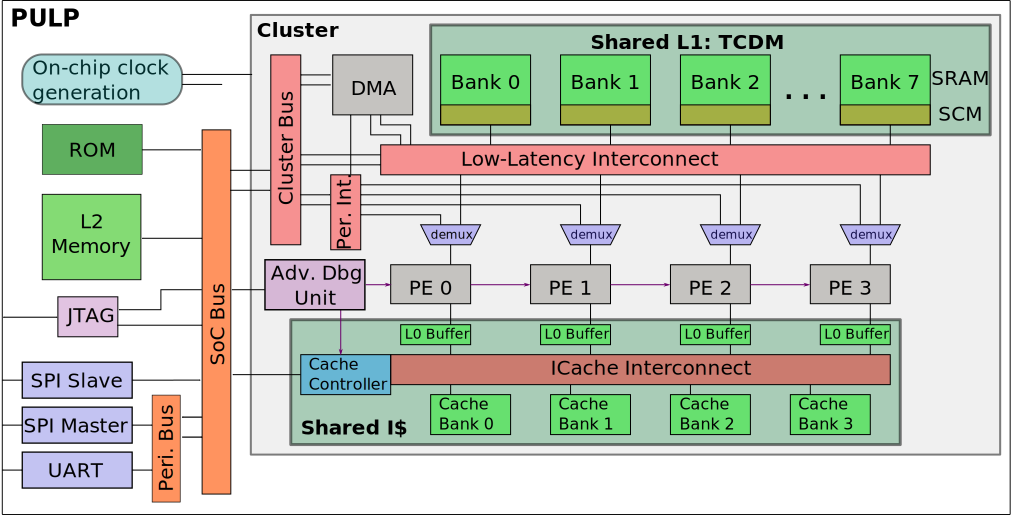
\includegraphics[width=0.9\textwidth]{./figures/PULP}
  \caption{PULP system overview.}
  \label{fig:pulp_overview}
\end{figure}

Until the beginning of this thesis \gls{PULP} was using a modified version of
the OR1200 OpenRISC core \cite{OR1200} that was created by the OpenRISC
community. During this thesis we switched the core to \orion, the core that we
developed solely for its use in \gls{PULP}.


\section{OR10N Core}

\orion is the OpenRISC core that replaces the previously used OR1200. \orion was
originally developed by Matthias Baer and Renzo Andri during a semester thesis
at ETHZ. It was already used in several chips, for example Sir10us
\cite{Sir10us} and \orion that were produced in 180 nm UMC technology and
successfully tested before we started integrating \orion into the \gls{PULP}
environment.

Prior to this thesis, the instruction set of \orion was enhanced with several
features that are not part of the OpenRISC specifications, specifically support
for hardware loops and auto-incrementing load and store operations, see
Section~\ref{sec:or10n_hwlp_prepost} for more details on the extensions.


\begin{figure}[htbp]
  \centering \includegraphics[width=0.9\textwidth]{./figures/or10n_overview}
  \caption{\orion general overview.}
  \label{fig:or10n_overview}
\end{figure}


\orion is based on a simple in-order four stage pipeline. In terms of core
energy efficiency an in-order single-issue processor design is the most
efficient \cite{azizi2010}. To achieve high \gls{IPC} values in such a core a
shallow pipeline with a low number of pipeline stages is important as this
reduces the number of possible data hazards.
The four pipeline stages of our \orion core are \gls{IF}, \gls{ID}, \gls{EX}
and \gls{WB}.

During the IF stage instructions get transferred from the instruction cache to
the core and the program counter is updated with the next value. If the
instruction cache can not immediately deliver the required instruction, the core
is stalled for the required amount of cycles.

The ID stage takes care of decoding instructions, performing accesses to the
register file and forwarding results to operands if they are needed in the next
cycle. Also the main control \glspl{FSM} reside in this stage.

The EX stage is the main computation stage in \orion. ALU and multiplication
operations are performed here and the results stored in the register file.
The address for a memory access is computed during the EX stage and sent to
the data memory interface.
If the address belongs to the \gls{TCDM} address space, data can be accessed in
a single cycle.
Otherwise a memory access will take multiple cycles and the core needs to be
stalled until the request has been served and the required data has been
delivered to the core.

During the \gls{WB} stage, the received data is multiplexed with \gls{SPR} data
and stored in the \gls{GPR}. The \gls{LSU} that is responsible for managing
memory accesses is part of the \gls{WB} stage and takes care of sign-extending
the received data and aligning it.
The \gls{SPR} that contains data that is important during the runtime of the
\gls{CPU}, is also part of the \gls{WB} stage. For example the arithmetic carry
and overflow flags are stored in the \gls{SPR} and can be accessed with
\instr{l.mfspr} instructions.

\orion uses a five port general-purpose register file with two write ports and
three read ports. One write port of the register file is used for ALU operations
exclusively, while the second write port is shared between SPR and memory
access. Two of the three read ports of the register file are used for normal \gls{ALU}
operations and memory accesses. The third read port is only used for two special
operations, namely the multiply-accumulate operation and register-register
store operations.

The final \orion core needs $44.5$ kGE area and achieves a clock period of
$2.23$ ns clock period in a UMC $65$ nm technology. The critical path in the
core is balanced between data memory address generation, the \gls{MAC} unit and
instruction fetch from the shared instruction cache.


\section{Compiler Support}

To write applications for the PULP platform we did not want to rely exclusively
on assembler as this makes development cumbersome and error-prone, instead C is
mainly used.
Thus to perform the translation from C to OpenRISC machine code a compiler is needed.
The OpenRISC community has already provided a port of \gls{GCC} to OpenRISC
which we reused for our system. But to get more performance and being able to
use our additional instructions, some changes to the compiler were needed to
actually emit those new instructions automatically. The researchers at
Politechnico di Milano did a port of the LLVM compiler to OpenRISC and added
support for our instruction set extensions to it.  This means that one can write
applications for PULP entirely in C and benefit from our \gls{ISA} extensions
automatically as there is full compiler support for it.

Writing parallel applications for a multi-core environment is difficult. To
simplify the development such applications, we ported OpenMP to our platform and
thus a programmer can take advantage of the constructs given by this framework.

%Eric Flamand has been working on adapting \gls{GCC} to the new instruction set
%that we have been developing. So our additional instructions are supported by
%both major compilers, \gls{GCC} and LLVM which allows us to make direct
%comparisons between the two.
%
%Both compilers are able to automatically emit code that uses the additional
%instructions and thus we can accelerate existing code without changing it.

%%% Local Variables: 
%%% mode: latex
%%% TeX-master: "../report_template"
%%% End: 

%%%%%%%%%%%%%%%%%%%%%%%%%%%%%%%%%%%%%%%%%%%%%%%%%%%%%%%%%%%%%%%%%%%%%%%
%%%%%%%%%%%%%%%%%%%%%%%%%%%%%%%%%%%%%%%%%%%%%%%%%%%%%%%%%%%%%%%%%%%%%%%
%%%%%                                                                 %
%%%%%     <file_name>.tex                                             %
%%%%%                                                                 %
%%%%% Author:      <author>                                           %
%%%%% Created:     <date>                                             %
%%%%% Description: <description>                                      %
%%%%%                                                                 %
%%%%%%%%%%%%%%%%%%%%%%%%%%%%%%%%%%%%%%%%%%%%%%%%%%%%%%%%%%%%%%%%%%%%%%%
%%%%%%%%%%%%%%%%%%%%%%%%%%%%%%%%%%%%%%%%%%%%%%%%%%%%%%%%%%%%%%%%%%%%%%%

\chapter{Related Work}

\label{chapter:related_work}


\section{Hardware Loops \& Auto-Incrementing Load/Stores}
\label{sec:or10n_hwlp_prepost}

The \gls{PULP} team has already extended the OpenRISC \gls{ISA} prior to this
thesis, i.e. zero-overhead hardware loops and extended addressing modes for load
and store operations were added.

Hardware loops eliminate the need of explicitly stating branch instructions
and decreasing the loop counter, instead this is done automatically by the
hardware when encountering the end of a given loop.
Hardware loops need to be set up beforehand with dedicated instructions. Those
instructions specify the begin and end of the loop and how many times it shall
be executed. During loop execution the core then takes care of jumping to the
beginning of the loop when the end is encountered and the loop counter has not
yet reached zero, while at the same time the loop counter is decremented.
When no hardware loops are used for a loop, an overhead of at least three
instructions is introduced, one instruction for decrementing the loop counter,
one for a set flag operations to check for the exit condition, one for
the branch instruction and maybe one instruction in the delay slot of the
branch. All those instructions are eliminated with hardware loops and thus we
gain on code size and execution speed.

As expected, this helps a lot when used on small loops, but less on
bigger ones. The cost and benefits of multiple hardware loop levels was
evaluated and it was decided that two levels of hardware loops are enough for
almost all applications. For some few applications an additional speedup can be
achieved by using even more levels, but this comes at a hardware cost which does
not justify the benefits.

Extended memory addressing modes were added to the core by implementing
auto-incrementing load and store operations and register-register addressing.
Auto-incrementing load and store instruction do not only perform a memory
access, but also take care of increasing the address by the amount specified as
offset and save it back to the register file. Two different modes of operations
are supported, pre-increments and post-increments. Pre-increments first
increase the address by the value specified in a register or immediate and use
the incremented address to access the memory, while post-increment instructions
address the memory directly with the base address and store the incremented
value in the register file.
Register-register addressing adds the possibility to specify a memory address as
an addition of register operand $A$ plus operand $B$ and allows much more
general memory access patterns than just register operand $A$ plus an immediate.
The operand $A$ plus immediate addressing mode was the only addressing mode
available in the OpenRISC base \gls{ISA}.

Since for auto-incrementing load operations two register values need to be
written at the same time, i.e. one for the modified address and one for the
value from memory, two write ports on the register file are required.
The typical register file of a \gls{RISC} CPU includes two read ports and one
write port which is not enough to perform two writes simultaneously. To solve
this problem, an additional write port was added to the register file. Since a
second port was already added when this thesis was started, we started using it
more aggressively during this thesis, i.e. all \gls{ALU} operations now use the
second write port of the register file per default while the first one is only
used for memory access and \gls{SPR} accesses, i.e. operations that are not
ready in the \gls{EX} stage of the core.

To implement register-register store instructions, three register values need
to be read at the same time, i.e. two for the address calculation and one to be
stored in memory. To accomplish this a third read port was added to the RF
which we then used during this thesis for new \gls{MAC} instructions as well.


\section{Vectorial Instructions}

Vectorial instructions aim to use the full potential of the 32 bit data path
when we are computing on data that is only 8 or 16 bit wide. We can segment the
data path into two or four parts and perform calculations on 2x 16 bits or 4x 8
bits in parallel. Those kind of operations are also known as sub-word parallelism
\cite{MAX2, PLX}, packed-SIMD \cite{RISCV} or micro-SIMD \cite{MCOMP} instructions.

It has been shown in \cite{PLX} that vectorial instructions can cut down the number
of cycles by a factor of four when operating on data that has 1/4th of
the width of the data path. 

Also \cite{MAX2} has implemented a set of vectorial instructions and show that
the overhead of partitioning the data path does not have a significant impact
on the area, timing or design time of a \gls{CPU}.
%They did not add support for vectorial multiplications since in their opinion
%having a multiplication with the same output width as they width of its input
%is not sufficient.


Most of the parallelism is available in addition, subtraction, averaging,
shifting, maximum, minimum, absolute number calculation and comparisons. Those
operations are frequent on 8 and 16 bit data types in multimedia applications
\cite{MCOMP} and thus one can expect a large speedup for this kind of
applications.

The OpenRISC specifications \cite{OR1KSPEC} already contain a proposal for
vectorial instructions for their 64 bit \gls{ISA}, but they were never
implemented. Since our core is based on 32 bits, it was not possible to directly
build on those specifications. Similarly we wanted to add additional features
that were not present in the original specifications done by the OpenRISC
community.

As a reference to our own vectorial instruction set, we checked what ARM offers
on their Cortex M4 \glspl{CPU} \cite{CM4UG}. For example they implement
vectorial addition, subtraction and averaging.
ARM also added extensions to the multiplier, e.g. they support sub-word
selection.
Sub-word selection multiplication instructions take two 32 bit operands A and
B.  For each of those 32 bit input operands the upper or lower 16 bits are
selected as input to the multiplier and thus a 16 bit times 16 bit
multiplication with a 32 bit result is performed.


RISC-V \cite{RISCV}, another open source instruction set similar to OpenRISC,
also aims to provide vectorial instructions. To this date no definite set of
instructions has been proposed, but they will add support for this kind of
instructions eventually. They also highlight one important point, when sub-word
parallel computation should be performed, it is desirable to have load and
store memory operations that support non-word aligned access.
The reason why it is desirable to support non-word aligned accesses is that if
vectorial operations are performed on data that is not aligned, the data
re-aligning for the vectorial instructions might eliminate the speedup. Also it
makes life much easier for a compiler since no special cases for non-aligned
memory accesses are necessary.
That misaligned memory access have a high performance impact was also shown by
\cite{UNALIGN} for the Altivec vector extensions.


%%%%%%%%%%%%%%%%%%%%%%%%%%%%%%%%%%%%%%%%%%%%%%%%%%%%%%%%%%%%%%%%%%%%%%%
%%%%%%%%%%%%%%%%%%%%%%%%%%%%%%%%%%%%%%%%%%%%%%%%%%%%%%%%%%%%%%%%%%%%%%%
%%%%%                                                                 %
%%%%%     04_vectorial.tex                                            %
%%%%%                                                                 %
%%%%% Author:      <author>                                           %
%%%%% Created:     <date>                                             %
%%%%% Description: <description>                                      %
%%%%%                                                                 %
%%%%%%%%%%%%%%%%%%%%%%%%%%%%%%%%%%%%%%%%%%%%%%%%%%%%%%%%%%%%%%%%%%%%%%%
%%%%%%%%%%%%%%%%%%%%%%%%%%%%%%%%%%%%%%%%%%%%%%%%%%%%%%%%%%%%%%%%%%%%%%%


\chapter{ISA Extensions}

\label{chapter:vectorial}

%The vectorial unit is supposed to increase the performance of the core when
%sub-word workloads are executed, e.g. operations on 8 or 16 bit numbers. Since
%\orion implements the 32 bit ISA of OpenRISC, it is possible to segment the data
%path, i.e. support 4x 8 bit or 2x 16 bit operations on the same data path
%without increasing the area of the data path by a significant amount.

%The OpenRISC specifications already contain a proposal for a vectorial
%extension on 64 bit \cite{OR1KSPEC}, called ORVDX64. We only have a 32 bit
%implementation and wanted to keep it that way, thus using ORVDX64 without
%modifications was not an option. Although we still used ORVDX64 as a basis for
%our own vectorial extension, adapted it to 32 bit, removed some instructions
%from it and added others.

This chapter describes the \gls{ISA} extensions that were integrated during this
thesis. Four sets of extensions were done, the first being a vectorial
extension to the \gls{ALU} which is detailed in Section~\ref{sec:vectorial}.
Section~\ref{sec:multiplier} explains the improvements to the \gls{MAC} unit of
the core. This includes adding vectorial support to the multiplier, sub-word
selection and more general multiply-accumulate instructions.
In Section~\ref{sec:misaligned_access} the misaligned memory access
implementation is explained.
Finally Section~\ref{sec:bit_count} explains the added bit counting instructions.

An overview over the encoding, mnemonics and semantic of the modified \gls{ISA}
is available in Appendix~\ref{chap:instr_encoding}.

\section{Vectorial Unit}
\label{sec:vectorial}

Our vectorial instructions extend the \gls{ALU} operations of the original
OpenRISC \gls{ISA}. In general every \gls{ALU} operation has two input operands
and one result that is stored in the general-purpose register file. There are
certain exceptions where an operation only has one input operand, e.g. for
example absolute number calculation which only needs one input operand.

\clearpage
For all instructions that take two operands, we have added six instruction
forms:

\begin{table}[H]
 \caption{Vectorial instruction forms.}
 \label{tab:vectorial_instr_forms}
 \centering\begin{tabular}{@{}lrl@{}} \toprule
  \textbf{Mnemonic} & \textbf{Width} & \textbf{Note} \\ \midrule
  lv.inst.h         & 16 bit         &  \\
  lv.inst.h.sc      & 16 bit         & scalar replication of operand B register \\
  lv.inst.h.sci     & 16 bit         & scalar replication of operand B immediate  \\
  lv.inst.b         &  8 bit         &  \\
  lv.inst.b.sc      &  8 bit         & scalar replication of operand B register \\
  lv.inst.b.sci     &  8 bit         & scalar replication of operand B immediate \\
  \bottomrule
 \end{tabular}
\end{table}

Scalar replication modifies the second operand of the instructions by
replicating the lower half word two times for the 16 bit case and the lowest
byte four times for the 8 bit case, i.e. it performs the following:
\begin{align*}
  opB[31:0] &= \{rB[15:0], rB[15:0]\} &\text{; 16 Bit case}\\
  opB[31:0] &= \{rB[7:0], rB[7:0], rB[7:0], rB[7:0]\} & \text{; 8 Bit case}\\
\end{align*}

Instead of replicating the register, the \textit{.sci} form replicates the
immediate encoded in the instruction. We have used an 8 bit wide immediate for
our vectorial instructions. For the 8 bit case the immediate is used directly,
while for the 16 bit case the immediate is sign-extended.

In the following sections an overview of the different \gls{ALU} operations is
given with details on how they were implemented.


\subsection{Addition / Subtraction / Average}

Addition and subtraction are the most basic features of an \gls{ALU} and among
the most used operations on 8 and 16 bit data types. Another common operation is
the average of two numbers, so we added support for this operation in our data
path as well. Averages were not supported in the original OpenRISC
specifications.

Figure~\ref{fig:alu_add_vec} shows the implementation of the vectorial addition,
subtraction and average. The same data path can be used for 8, 16 and 32 bit
operations. The only overhead introduced by vectorial instructions four 1-bit
wide multiplexers that are placed between the 8 bit adder slices and take care
of handling the carry bit correctly between the different slices.  On the right
hand side of this figure the additional hardware that was needed to perform
averages is shown. An average is computed by first adding the two operands and
then performing an arithmetic right shift by one bit. Note that the arithmetic
right shift performs a division by 2 towards negative infinity.

\begin{figure}[htbp]
  \centering
  \includegraphics[height=1.0\textwidth,angle=270]{./figures/alu_add_vec}
  \caption{Vectorial addition/subtraction.}
  \label{fig:alu_add_vec}
\end{figure}

% lv.add
% lv.sub
% lv.avg

\subsection{Minimum / Maximum / Absolute Value}

Calculating minimum, maximum and absolute values is important for many
applications. Using the standard OpenRISC instruction set those operations need
a lot of instructions including branches. 
Our main interest lay on vectorial instructions, but since we wanted those
instructions for the vectorial unit, we were able to also add them to the normal
integer pipeline without any additional cost, thus we introduced the following
instructions that were not part of the original OpenRISC instruction set:
\instr{l.min}, \instr{l.max} and \instr{l.abs}.

Figure~\ref{fig:max_inst} shows a comparisons of assembler instructions
necessary to perform a maximum computation. On the left an optimized maximum
computation based on the original OpenRISC specifications can be found. Note
that a compiler would usually use at least five instructions to perform the
same operation as it is not able to put the first addition into the delay slot.
On the right hand side the same functionality is shown with our new max
instruction.  When we consider many maximum calculations on sub-word integers,
the strength of having a dedicated maximum instruction gets even more pronounced
because the vectorial version can be used.

% Create an enviroment for shell commands.
\newenvironment{shellenv2}%
{%
   \begin{Sbox}\begin{minipage}{\textwidth}\begin{texttt}%
 }%
 {\end{texttt}\end{minipage}\end{Sbox}%
 \setlength{\fboxsep}{6pt}\shadowbox{\TheSbox}}%


\begin{figure}[H]
 \begin{subfigure}[b]{0.45\linewidth}
\begin{instrenv}
l.sfgts rA, rB
l.bf 0xC
l.addi rD, rA, 0
l.addi rD, rB, 0
\end{instrenv}
  \caption{Original max. computation.}
 \end{subfigure}\hfill
 \begin{subfigure}[b]{0.45\linewidth}
  \begin{instrenv}
l.max rD, rA, rB
  \end{instrenv}
  \caption{New max. instruction.}
 \end{subfigure}

 \caption{Maximum operation in assembler.}
 \label{fig:max_inst}
\end{figure}


Figure~\ref{fig:alu_minmax} shows the implementation of the min/max/abs circuit.
Since this operation was not present in the \orion core before this thesis has
started, we had to add additional hardware. Mainly what was needed was a
vectorial comparison unit (which was also needed for vectorial comparison
operations) and a multiplexer on 32 bit.

If we consider only the maximum operation, the circuit works as follows.
The two operands, \textit{op\_a} and \textit{op\_b}, are fed into a vectorial
comparison unit that is configured based on the vectorial mode (8, 16 or 32 bit)
and signed mode. The output of the vectorial comparator is then used to set the
multiplexers to the correct setting and select the bigger of the two operands.
This works almost exactly the same way for minimum, the only difference being
that the output of the vectorial comparator is inverted and thus instead of the
bigger of the two operands the smaller is chosen.

To perform an absolute value calculation, we reuse the subtraction of the
vectorial adder that was described above. In this case \textit{op\_a} is the
operand data, while \textit{op\_b} is set to 0. The adder then computes $0 -
\textit{op\_a}$ and supplies this result to \textit{res\_sub}.  The vectorial
comparator compares \textit{op\_a} and 0, and using this result we can select
either \textit{op\_a} or $-\textit{op\_a}$ with the multiplexers.

\begin{figure}[htbp]
  \centering
  \includegraphics[height=1.0\textwidth,angle=270]{./figures/alu_minmax}
  \caption{Vectorial min/max/abs.}
  \label{fig:alu_minmax}
\end{figure}




\subsection{Shifts}

Similar to other implementations \cite{PLX,MAX2} we wanted to support vectorial shift
instructions because a considerable part of today's workloads involve shift
operations on sub-word data. For those instructions shifts by immediates and
shifts by values stored in registers should be supported which is a very good
fit for our instruction format described in
Table~\ref{tab:vectorial_instr_forms}.

Vectorial shift operations with scalar replication of immediates shifts all
sub-words by the same amount to the left or right. The same is true for scalar
replication of registers. But if scalar replication is not used, it is possible
to shift each sub-word of operand A by a different amount given by the sub-words
in operand B. Allowing shifts by different amounts in a vectorial operation
makes it more general and allows the use of the vectorial unit in more cases.

If shift operations would not be supported, it would sometimes be necessary to
convert the vector data type to multiple scalar data values to perform those
operations. In many cases this would ruin the performance gains that were
achieved by using other vectorial instructions.
In the end it would be better not to use vectorial instructions at all in those
cases.

%TODO: implementation


\subsection{Logical Operations}

To support logical operations for vectorial workload nothing has to be added in
hardware, since an \instr{AND} on 8 or 16 bit is identical to an \instr{AND} on
32 bit. The only difference being that our design for vectorial instructions
allows scalar replication. Since this was already implemented for other
vectorial operations, adding scalar replication for logical operations was
entirely for free in hardware.

The following logical operations have been added without any hardware overhead
except for the necessary decoding of the new instructions:
\begin{itemize}
  \item \instr{lv.and\{,.sc,.sci\}}
  \item \instr{lv.or\{,.sc,.sci\}}
  \item \instr{lv.xor\{,.sc,.sci\}} 
\end{itemize}



\section{Multiplication}
\label{sec:multiplier}

One of the most critical operations in a typical RISC pipeline is the
multiplication, its operation is far more complex than an addition and it
thus has a much higher delay, even when considering vectorial additions.

To keep the common case fast in the core, we decided to simplify the
multiplication design and try to fit it into just one cycle. The original OR1200
core used three cycles to compute a multiplication \cite{OR1200}, while the
original \orion core used two cycles because the full 64 bit result could not be
computed in a single cycle without impacting the critical path.

For the applications we are targeting the 64 bit result of a multiplication is
of minor importance, so we decided to move to a 32 bit result in order to
simplify the hardware design. Multiplying a 32 bit number with a 32 bit number
now yields the lower 32 bit of the product  in our modified ISA instead of the
full 64 bit wide product.
While we loose precision and cannot incorporate the full 64 bit result, we gain
performance as it is simpler to calculate only a 32 bit product. The 64 bit
result of a multiplication is seldom used and it is cumbersome to obtain in
OpenRISC as it is not saved in a \gls{GPR} but in a \gls{SPR}. In order to
use the result in the original OpenRISC specifications, one would have to first
move it from the \gls{SPR} to the \gls{GPR} using two \instr{l.mfspr}
instructions. As the \gls{SPR} is part of the \gls{WB} stage of the core, the
two \instr{l.mfspr} instructions may take three cycles if the result should be
used in the next cycle, this is due to a necessary pipeline stall in this case.
So together with the two cycle execution of the multiplication we end up with a
five cycle latency to compute a 64 bit result and use it for normal operations.


\subsection{(Vectorial) MAC}
The \gls{MAC} operation that is specified in OpenRISC \cite{OR1KSPEC} uses a 64
bit wide accumulator stage. Since a \gls{MAC} operation needs three input
operands to perform the operation $d \mathrel{{+}{=}} a \cdot c$, the
accumulator is kept local in the \gls{SPR} to hold the 64 bit wide operand $d$.
To transfer data between the general-purpose and the special-purpose registers a
significant overhead is required and many cycles are lost due to this, i.e. two
cycles to initialize the \gls{SPR} and two to three cycles to get the result
back to the \gls{GPR}. This is especially bad when only one \gls{MAC} operation
on 32 bits is required, in this case it is better to just perform a
multiplication and a subsequent addition in two separate instructions instead of
using the dedicated \gls{MAC} instruction which would need a total of five
cycles.

In order to get rid of this issue, we added another \gls{MAC} instruction which
uses the general-purpose register as the source of the accumulator. This fits
very well with the 32 bit result of the multiplier, as the general-purpose
registers are only 32 bit wide.
By moving to this scheme and still perform one \gls{MAC} operation per cycle, we
needed a register file with three read ports, two for the operands A and B and
one for the accumulator. Since a third read port was already introduced for the
register-register store operations, this did not add any additional hardware
overhead.
%This led to a register file with three read ports and two write ports as an
%additional write port was added due to auto-incrementing loads and stores.
%This is of course larger than the normal register file in a \gls{RISC} processor
%that has only two read ports and one write port.

To get the full set of \gls{ALU} operations also in the vectorial case, there
needs to be support for performing 4x 8 bit and 2x 16 bit multiplications. The
output range of those multiplications is limited to 8 bit, 16 bit respectively,
but there are still applications that can benefit from such instructions.
As we have already decided to have a \gls{MAC} instruction that uses the
general-purpose register to store the accumulator, we could also do this for the
vectorial case.


Comparing the original OpenRISC specifications with our extension, we removed
multiply-accumulate on 64 bit with the accumulator in \gls{SPR} and use a
general-purpose register file based accumulator instead. We add vectorial
operations to the \gls{MAC} unit and allow 4x 8 bit and 2x 16 bit
multiplications in parallel.


\subsection{Sub-Word Selection}

To support multiple precision multiplications, e.g. 32 bit number times 32 bit
number with a 64 bit wide product, in an efficient manner, we needed some additional
instructions. Getting a 64 bit result for a 32 bit x 32 bit multiplication was
easy with the original OpenRISC specifications, but not so simple anymore when
we have limited the output range of the multiplier to the lower 32 bit.

To mitigate this issue, sub-word selection for multiplications was introduced.
With only a 32 bit multiplication result, full precision can only be achieved
when 16 bit input operands are used. To calculate a 64 bit multiplication
product, four partial products have to be computed and added in subsequent
steps. Figure~\ref{fig:mul64_instructions} shows the assembler instructions
necessary to perform the 64 bit multiplication.
Figure~\ref{fig:mul64_original} shows the case when we follow the OpenRISC
specifications which needs at least four cycles to execute, depending on
pipeline stalls of the implementation.
Figure~\ref{fig:mul64_wo_spr} shows the case when we use only a 32 bit result of
the multiplier. To compute the 64 bit product four 32 bit wide partial products
are needed. Each partial product is computed by performing one 16 bit times 16
bit multiplication. The four partial products are then shifted accordingly and
accumulated. Since the result spans two general-purpose registers, care must be
taken to handle the carry between the two 32 bit registers correctly. This
computation needs 16 instructions in total and thus 16 cycles are required.

Sub-word selection allows us to select the lower or upper 16 bits of both input
operands of the multiplier before performing the multiplication or \gls{MAC}
operation. This means we can perform for example
$$
rC[31:0] + \big(extZ\left(rA[15:0]\right) \cdot extS\left(rB[31:16]\right)\big)
$$
in one cycle.
So if we reconsider the 64 bit multiplication from above and use sub-word
selection and the general-purpose register \gls{MAC} instruction, we can go down
to 10 instructions and thus only 10 cycles to calculate a 64 bit product.

Sub-word selection is not only useful for a 32 bit times 32 bit multiplication,
but also for much wider multiplications, i.e. multiple-precision
multiplications.

%TODO: talk about multiple-precision algorithms with the new MAC

\begin{figure}[H]
 \begin{subfigure}[b]{0.30\linewidth}
   \footnotesize
   \begin{instrenv}
l.muld  rA, rB
l.mfspr rD, MACLO
l.mfspr rE, MACHI
   \end{instrenv}
  \caption{Original.}
  \label{fig:mul64_original}
 \end{subfigure}\hfill
 \begin{subfigure}[b]{0.30\linewidth}
   \footnotesize
   \begin{instrenv}
l.andi t0, rA, 0xFFFF
l.andi t1, rB, 0xFFFF
l.sra  t2, rB, 16
l.sra  t3, rB, 16
l.mul  t4, t0, t3
l.sll  t5, t4, 16
l.sra  t4, t4, 16
l.mul  t6, t0, t1
l.mul  t7, t2, r3
l.add  t5, t5, t6
l.addc t4, t4, t7
l.mul  t6, t1, t2
l.sll  t0, t6, 16
l.sra  t1, t6, 16
l.add  t4, t4, t0
l.addc t5, t5, t1
   \end{instrenv}
  \caption{w/o SPR.}
  \label{fig:mul64_wo_spr}
 \end{subfigure}\hfill
 \begin{subfigure}[b]{0.33\linewidth}
   \footnotesize
   \begin{instrenv}
l.mul.sh.zl  t0, rA, rB
l.sll        r1, t0, 16
l.srl        r2, t0, 16
l.mac.zl.zl  r1, rA, rB
l.macc.sh.sh r2, rA, rB
l.mul.sh.zl  t0, rB, rA
l.sll        t1, t0, 16
l.srl        t0, t0, 16
l.add        r1, r1, t1
l.addc       r2, r2, t0
   \end{instrenv}
  \caption{with subword selection.}
  \label{fig:mul64_subword}
 \end{subfigure}

 \caption{64 bit multiplication with different hardware support.}
 \label{fig:mul64_instructions}
\end{figure}

Sub-word selection can also be used for vectorial operations, e.g. we have input
data arranged in two 16 bits inside one 32 bit word and we would like to
calculate a 16 bit times 16 bit multiplication with a 32 bit result. Following
the OpenRISC specifications we first have to shift the inputs by 16 bit to the
right to get only the higher 16 bits or perform an AND operation to get only the
lower 16 bits respectively. With our new feature, we can omit this pre-processing
and perform the multiplication directly, thus making it more efficient.


\subsection{Implementation}

For the implementation of the vectorial multiplier several alternatives were
evaluated, namely using a vectorial booth multiplier \cite{BoothMul}, shared
segmentation \cite{SharedSeg} and a pure behavioral specification in
SystemVerilog.


\subsubsection{Vectorial Booth Multiplier}

The circuit shown in Figure~\ref{fig:vectorial_booth_mult} is able to perform
vectorial multiplication and \gls{MAC} operations, normal 32 bit multiplications
and \gls{MAC} calculations with 32 bit result. It uses four booth multipliers
with different input and output widths. The width of the first operand of each
booth multiplier is set to 8, 16, 24 and 32 bits respectively, while the
second operand is always 8 bit wide. The output of those multipliers is a
8, 16, 24 or 32 bit number in carry save number format, i.e. two 32 bit signals
are used to represent one 32 bit number. By feeding the results of the booth
multipliers into 4:2 compressors and shifting them accordingly, we can get the
normal 32 bit result. By adjusting the multiplexers in front of the booth multipliers
and the final multiplexer before the partitioned adder correctly, we can get the 4x 8
bit and 2x 16 bit results as well. The partitioned adder then finally takes care
of performing the addition of the carry save number and transforming it into a
normal integer that can be saved into the register file later on. The
partitioned adder takes care of suppressing carries between 8 bit and 16 bit
boundaries if the 4x 8 bit or 2x 16 bit vectorial modes are used.

\begin{figure}[H]
  \centering
  \includegraphics[height=1.0\textwidth,angle=270]{./figures/booth_mult}
  \caption{Vectorial booth multiplier.}
  \label{fig:vectorial_booth_mult}
\end{figure}

The booth multiplier and 4:2 compressors were implemented by using DesignWare
components available from Synopsys \cite{DW}, specifically \texttt{DW02\_multp}
for the booth multiplier and \texttt{DW02\_tree} for the compressors. We also
tried to implement the booth multiplier and 4:2 compressors directly but the
results of using DesignWare components were a few percent better in terms of
area and delay.


\subsubsection{Shared Segmentation}

Shared segmentation is another possibility to implement a fast vectorial
multiplier. It is based on the idea to generate the partial products in the
right bit positions from the start, also in the vectorial case. For the booth
multiplier mentioned above, multiplexers and shifts are needed to align the partial
products correctly. Shared segmentation takes care of those issues at the
beginning of the calculation by emitting them in the correct bit positions of
the partial product already. This allows a simplification of the reduction step,
where the 32 partial products are reduced to the final integer. The reduction
step in shared segmentation only needs Wallace tree adders with the option to
suppress carries between 8 and 16 bit boundaries for the vectorial modes.

More details about this method can be found in \cite{SharedSeg}.

% TODO: how implemented? probably too much work for too little reward...



\subsubsection{Behavioral}

Instead of writing complex multiplier implementations in SystemVerilog, we also
tried to do a very simple implementation by specifying the vectorial multiplier
in one \texttt{always\_comb} block in SystemVerilog. By packing the complete
functionality in just one block, we leave the synthesis tool the freedom to
choose the most suitable multiplier architecture. When we started with the
comparison of the different multiplier implementations, it was not yet clear
which one would be the best. We expected a purely behavioral implementation to
be worse, but instead the results were surprisingly good.



\subsubsection{Results \& Conclusion}

The different implementations were synthesized for the 28 nm FDSOI process of
STMicroeletronics that will be used for the pulp3 chip. The slow corner on $0.6$
Volts was used for the timing analysis, see Table~\ref{tab:mult_syn} for the
results.
Baseline is the implementation that was present before we started modifying the
\gls{MAC} unit, i.e. a two-cycle \gls{MAC} with 64 bit result that writes its
result into the special-purpose registers.

It can be seen that sub-word selection adds $\sim 0.06$ ns delay to the design, which
is in the order of only one gate delay. So we decided to accept this loss in
speed for having more features. Surprisingly the behavioral implementation seems
to be the fastest and when comparing the areas of the different implementations
it is also very competitive.
This is the reason why we decided to go with the behavioral implementation, as
it has a very simple SystemVerilog implementation and it is the fastest
available.

\begin{table}[H]
 \caption{Vectorial multiplier synthesis results.}
 \label{tab:mult_syn}
 \centering\begin{tabular}{@{}llrrr@{}} \toprule
  \textbf{Design}      & \textbf{Features} & \textbf{Area \orion [kGE]} & \textbf{Area Mult. [kGE]} & \textbf{Timing} \\ \midrule
  Baseline             & OR1k spec.        &             $41.1$ &              $12.2$ &       $7.57$ ns \\
  Vec. Booth Mult.     & MAC               &             $38.5$ &              $10.7$ &       $7.83$ ns \\
  Vec. Booth Mult.     & MAC, subword      &             $38.5$ &              $11.1$ &       $7.83$ ns \\
  Shared Segmentation  & MAC               &             $39.8$ &              $13.6$ &       $7.77$ ns \\
  Shared Segmentation  & MAC, subword      &             $38.5$ &              $10.5$ &       $7.84$ ns \\
  Behavioral           & MAC               &             $38.6$ &               $8.6$ &       $7.58$ ns \\
  Behavioral           & MAC, subword      &             $38.6$ &               $8.8$ &       $7.64$ ns \\
  \bottomrule
 \end{tabular}
\end{table}



\section{Misaligned Memory Access}

\label{sec:misaligned_access}

Misaligned memory access represents the case when a memory load or store
operation is performed that is not aligned on a natural word address. Since our
whole memory subsystem is word-organized, this case is difficult to handle. This
is the reason that the OpenRISC specifications do not allow non-word aligned
memory access, or misaligned accesses as we will call them from now on. But
there are certain benefits to add support for this kind of memory transaction,
especially vectorial operations can gain a lot of performance, since it is very
probable that we compute on 8 or 16 bit data that is not aligned on a word
address. Figure~\ref{fig:unaligned_mem_access_5x5} shows a use case of
misaligned memory access where we want to put a filter on a 2D image. The
unaligned word on the right hand side needs two load words, two shifts and one
OR instruction if no misaligned accesses are supported. So in the end it might
happen that more cycles are needed to prepare the data than what we can gain
with our vectorial operations, so it might be better to stick to conventional
operations.

\begin{figure}[htbp]
  \centering
  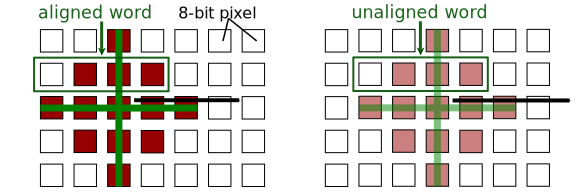
\includegraphics[width=0.7\textwidth]{./figures/unaligned_mem_access_5x5}
  \caption{2D filter with misaligned words.}
  \label{fig:unaligned_mem_access_5x5}
\end{figure}

Figure~\ref{fig:misaligned_access} shows a comparison of assembler instructions
necessary for performing a misaligned access when it is supported by the
hardware and when it is not supported. The effect on code density is immediately
visible and it is obvious that with hardware support the load can be performed
much faster.

\begin{figure}[H]
 \begin{subfigure}[b]{0.45\linewidth}
\begin{instrenv}
l.lwz  rD, 0(rA)
l.lwz  t0, 4(rA)
l.srli rD, rD, 0x1
l.slli t0, t0, 0x1
l.or   rD, rD, t0
\end{instrenv}
  \caption{w/o support.}
 \end{subfigure}\hfill
 \begin{subfigure}[b]{0.45\linewidth}
\begin{instrenv}
l.lwz rD, 1(rA)
\end{instrenv}
  \caption{with support.}
 \end{subfigure}

 \caption{Misaligned access.}
 \label{fig:misaligned_access}
\end{figure}

\gls{PULP} uses a word-aligned memory subsystem, therefor if we want to add
support for this kind of memory access, we have to do it in the core itself or
modify the memory subsystem. Preliminary trials on modifying the memory
subsystem resulted in an increase of about 10\% of our target clock period
which is not justifiable as it is only a corner case. Supporting misaligned
memory accesses in the \gls{LSU} of the core on the other hand does not impact
the timing.

Supporting misaligned memory access in the core means that two load operations
need to be performed to get the two words from the memory that contain our
misaligned word. In \orion we added support for misaligned accesses by handling
them directly in the load-and-store unit. This unit stalls the core when it
detects a misaligned load, performs the first memory access, saves the result
in a register, then performs the second load and finally assembles the complete
word from the two words. During this time the rest of the core is stalled, so
loading a misaligned word is slower than loading an aligned word, but since
everything is performed in hardware, we are only getting the delay of loading
two words and not the additional overhead of the shifts and OR operations that
are needed when there is no support in hardware. This means that in the best
case a misaligned access can be performed in just two cycles, compared to the
five cycles that were needed previously.
Of course the implementation for storing a misaligned word in memory is very
similar and also only takes two cycles in the best case.

There are not so many use cases for misaligned memory accesses in conventional
code, since the compiler always tries to align the data to natural word
boundaries. But in the case of vectorial operations, the compiler gets much more
freedom. So this is why a performance improvement can be seen by having support
for misaligned accesses when using vectorial operations.

%TODO: say that this is very important


\section{Bit Counting Instructions}

\label{sec:bit_count}

Bit counting instructions are instructions that work on the bit level of a
single word, e.g. counting the number of bits set to $1$ or $0$ in a word,
finding the first bit set to $1$ starting from the \gls{LSB} and so on.
OpenRISC \cite{OR1KSPEC} already specifies the instructions \instr{l.ff1} and
\instr{l.fl1}, but those instructions were not yet implemented in \orion.

During this thesis we added support for a couple of those kind of instructions.
Specifically we added the following instructions:

\begin{itemize}
  \item \instr{l.ff1}: Find first bit set to $1$ in a word starting from
    \gls{LSB}.
  \item \instr{l.fl1}: Find first bit set to $1$ in a word starting from
    \gls{MSB}.
  \item \instr{l.cnt}: Count the number of bits set to $1$ in a word.
  \item \instr{l.clb}: Count leading bits, the number of bits set to the same
    value as the sign bit.
\end{itemize}

It is obvious that those instructions are far more efficient than performing
those operations in the normal way using loops and branches. For example the
\instr{l.cnt} instruction would need more than 100 cycles to execute without
hardware support.

Table~\ref{tab:bit_count_syn} shows the area cost of the different
implementations compared to the baseline which does not include any of those
instructions. For this comparison the 28nm FDSOI technology from
STMicroeletronics was used. The baseline already includes the vectorial
instructions that were introduced above.
In total less than $15\%$ of the area of the \gls{ALU} is needed for all bit
counting instructions while the \gls{ALU} only occupies about $15\%$ of the area
of the core, so the area impact on the core is only about $2\%$ for all bit
counting instructions together. Similarly the bit counting instructions have no
impact on the timing properties of the core.


\begin{table}[H]
 \caption{Bit counting implementation}
 \label{tab:bit_count_syn}
 \centering\begin{tabular}{@{}lcc@{}} \toprule
   \textbf{Design}      & \textbf{Area ALU [GE]} & \textbf{ALU Percentage of Core Area} \\ \midrule
  Baseline             &           $6530$        & 13.3\% \\
  FF1, FL1             &           $6870$        & 14.0\%\\
  FF1, FL1, CLB        &           $6920$        & 14.1\%\\
  FF1, FL1, CLB, CNT   &           $7480$        & 15.3\%\\
  \bottomrule
 \end{tabular}
\end{table}

Considering a \gls{PULP} cluster with four cores, the area impact of bit counting
instructions becomes completely negligible. Such a cluster needs an area of
around $1500$ kGE, while all bit counting instructions together require only $1$
kGE, meaning that they have an impact of less than $0.07\%$ on the cluster area.

%%%%%%%%%%%%%%%%%%%%%%%%%%%%%%%%%%%%%%%%%%%%%%%%%%%%%%%%%%%%%%%%%%%%%%%
%%%%%%%%%%%%%%%%%%%%%%%%%%%%%%%%%%%%%%%%%%%%%%%%%%%%%%%%%%%%%%%%%%%%%%%
%%%%%                                                                 %
%%%%%     <file_name>.tex                                             %
%%%%%                                                                 %
%%%%% Author:      <author>                                           %
%%%%% Created:     <date>                                             %
%%%%% Description: <description>                                      %
%%%%%                                                                 %
%%%%%%%%%%%%%%%%%%%%%%%%%%%%%%%%%%%%%%%%%%%%%%%%%%%%%%%%%%%%%%%%%%%%%%%
%%%%%%%%%%%%%%%%%%%%%%%%%%%%%%%%%%%%%%%%%%%%%%%%%%%%%%%%%%%%%%%%%%%%%%%


\chapter{Debug Support}

\label{chapter:debug}

Being able to attach an external debugger to a \gls{CPU} is a crucial feature
in a modern \gls{SoC}. It is much more convenient to have access to internal
registers of the target, being able to add breakpoints and so on instead of
resorting to debug with printf and \gls{LED} flashing.
At the beginning of this thesis \orion lacked even basic debugging features, so
one of our goals was to add support for them.

There are many features one can support in a debug unit inside a \gls{CPU}. Among
them are single-stepping, hardware breakpoints on instruction addresses,
watchpoints and breaks on specific memory accesses. The OpenRISC specifications
\cite{OR1KSPEC} contain proposals for all of them, but adding support for all
those features would increase the complexity and area of our core
significantly and would make timing closure more difficult. For most of our
use cases we don't need such sophisticated features.
Especially breakpoints on memory accesses add a lot of complexity in hardware as
the core needs to stall (and flush) the entire pipeline as soon as a specific
address is encountered. The exact memory access address is only available in the
\gls{EX} stage when the request is sent towards the memory, so if such a request
should be inhibited due to the breakpoint, the delay for each access will
definitely be increased. In order to keep the complexity at a reasonable level
and avoid inflating the critical path, we decided to not add support for memory
breakpoints.

Watchpoints are an advanced feature of the debug unit which allow complex
breaking conditions. For example it is possible to break the program flow and
trap to the debugger when the program counter has a value between \texttt{0x1C023000} and
\texttt{0x1C02F000}, the program counter has hit the address \texttt{0x1C02E028}
exactly 5 times and the core currently tries to access memory address
\texttt{0x10004304}.
Supporting such sophisticated watchpoints adds on area and power consumption of
the core. Since this kind of functionality is seldom used, it is better to not
support it and save on area and power.


\section{Software Breakpoints}

We also did not add support for hardware breakpoints, i.e. breakpoints on
instruction addresses, instead we decided to rely solely on software based
breakpoints. Software breakpoints are specific instructions inserted into the
instruction stream which cause a trap to the debugger. Those trap instructions
(\instr{l.trap}) replace a normal instruction in the instruction stream and thus
after the breakpoint has been handled and execution continues, the original
instruction has to be reinserted into the instruction stream and executed by the
core. Figure~\ref{fig:debug_instr} shows this procedure. The arrow marks
the position of the program counter in the machine code after each step.
In step 1 the software breakpoint is inserted and program execution continues
until it hits the trap instruction. Now control is handled over to the debug
unit which can access the complete state of the core.
After we are done with debugging at this breakpoint, we continue execution and
go to step 2. In this step the trap instruction is replaced with the original
instruction and the program counter is set to point to it, so that it can be
executed as if there was no software breakpoint. To be able to set the software
trap again, we set the core into single-stepping mode, i.e. after each
executed instruction we trap to the debugger.
After control is handled over to the core again, it starts executing the
original instruction and traps to the debugger immediately after this
instruction because of the single-stepping mode.
In step 3 the debugger then reinserts the trap instruction and unstalls the core
so that program execution can continue.

\begin{figure}[htbp]
  \centering
  \includegraphics[width=0.9\textwidth]{./figures/debug_instr}
  \caption{Software breakpoints.}
  \label{fig:debug_instr}
\end{figure}

Having to replace instructions means a performance penalty during debugging
compared to hardware breakpoints, but on the other hand we add a lot of
flexibility. One can only have a very limited number of hardware breakpoints,
e.g. four, while we can have an unlimited number of software breakpoints. Since
one does not care much about performance when debugging software, flexibility is
far more important. Also hardware breakpoints involve a significant hardware
overhead for the registers that hold the breakpoint values and the arithmetic
that is needed to perform the actual instruction address comparisons.

There are several things to note about software breakpoints. Since instructions
are being replaced and our platform uses an instruction cache, we have to flush
this cache every time we make modifications in the code. Also we do not support
trap instructions in branch delay slots, so the debugger has to avoid placing
trap instructions there.




\section{OR10N Register Access}

Accessing general-purpose and special-purpose registers inside \orion is done
through existing read and write ports of the respective register files, see
Figure~\ref{fig:or10n_debug}. The changes required for debug support are
highlighted in red.

Since we multiplex those ports with signals that are in active use by the core,
we first have to put the core into a special mode before we are allowed to
access the registers. We do this by stalling it through the debug unit inside
\orion. Once the core is stalled, it is possible for the debugger to read and
write values.

\begin{figure}[htbp]
  \centering
  \includegraphics[height=0.9\textwidth,angle=270]{./figures/or10n_debug}
  \caption{\orion debug overview.}
  \label{fig:or10n_debug}
\end{figure}


\section{External Connection}

Attaching a debugger to the system involves several parts of the \gls{SoC},
i.e. one needs a protocol to communicate with the \gls{ASIC}, a way to signal
commands to the individual cores of the system and way to access the cores
separately.
For the first part, communication with the \gls{SoC}, we rely on the \gls{JTAG}
protocol. Via \gls{JTAG} the debugging system communicates with the advanced
debugging unit which takes care of high-level commands like determining if the
\gls{CPU} is stalled or if it is running. Finally the advanced debug unit
communicates with the \orion core to get access to general-purpose and
special-purpose registers and setting the program counter.
Figure~\ref{fig:debug} shows an overview over the complete system.

It is possible to debug the cores independently from each other, or halt
executing of all cores at the same time by setting up specific rules inside the
advanced debug unit. The advanced debug unit also takes care of communication
with the memories of the \gls{SoC} and is able to flush the instruction cache
via memory mapped registers after it has replaced instructions for software
breakpoints. In the final PULP system with multiple clusters there will be one
advanced debug unit in each cluster which is responsible for debugging of the
cores within that cluster.

\begin{figure}[htbp]
  \centering
  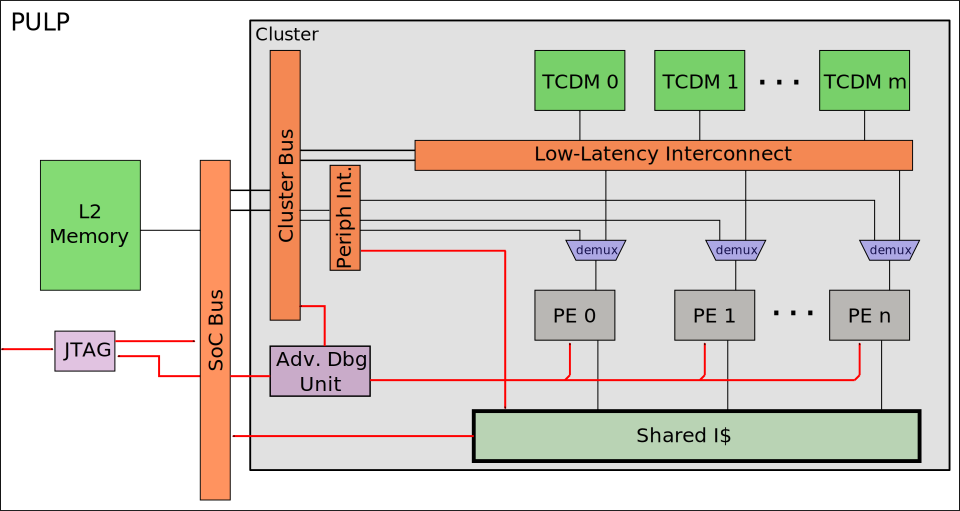
\includegraphics[width=0.9\textwidth]{./figures/debug}
  \caption{PULP debug overview.}
  \label{fig:debug}
\end{figure}

%%%%%%%%%%%%%%%%%%%%%%%%%%%%%%%%%%%%%%%%%%%%%%%%%%%%%%%%%%%%%%%%%%%%%%%
%%%%%%%%%%%%%%%%%%%%%%%%%%%%%%%%%%%%%%%%%%%%%%%%%%%%%%%%%%%%%%%%%%%%%%%
%%%%%                                                                 %
%%%%%     07_changes.tex                                              %
%%%%%                                                                 %
%%%%% Author:      <author>                                           %
%%%%% Created:     <date>                                             %
%%%%% Description: <description>                                      %
%%%%%                                                                 %
%%%%%%%%%%%%%%%%%%%%%%%%%%%%%%%%%%%%%%%%%%%%%%%%%%%%%%%%%%%%%%%%%%%%%%%
%%%%%%%%%%%%%%%%%%%%%%%%%%%%%%%%%%%%%%%%%%%%%%%%%%%%%%%%%%%%%%%%%%%%%%%

\chapter{Microarchitectural Changes}

\label{chapter:changes}



\section{Interrupts and Exceptions}


At the beginning of this thesis PULP was in the process of being switched from
the OR1200 core to \orion, thus at this point the new \orion core was $100\%$
backward compatible with the OpenRISC specifications \cite{OR1KSPEC}.  During
this thesis we started to deviate from those specifications, for example we
replaced the multiplier through a completely different implementation with more
features, that is not $100\%$ compatible with the original specifications
anymore.

In PULP we focus on energy efficiency and thus we need to be able to shutdown
the core when it is not in use, e.g. when it is waiting for the \gls{DMA} to
finish its job. For this purpose we are using events, a mechanism that puts the
core to sleep and wakes it up as soon as the event has happened, e.g. the
\gls{DMA} has finished.

We implemented this by having a separate event unit outside of the core that
takes care of clock gating of the core when it is asleep and waking it up
again. Since we already have this event unit outside the core which has access
to all event/interrupt sources, we did not want to duplicate this functionality
again in the core for an interrupt controller. Instead we decided to move the
interrupt unit out of the core into the event unit which contradicts with the
OpenRISC specifications that specify a programmable interrupt controller with
direct access to the special-purpose registers and is thus more tightly coupled
to the core than our implementation.

Interrupts are less important than events for a core that mostly performs
computations and seldom has to communicate with peripherals, thus we settled on
a very simple scheme to handle interrupts in \orion. In many big commercial
\glspl{CPU} one can find nested vector interrupt controllers, multiple register
file banks to be able to handle interrupts in a very fast way, adjustable
interrupt priorities and so on.

We wanted none of that but only the most basic functionality for our interrupt
system and we wanted to share most of this functionality also with exceptions to
keep the area requirements of the combined interrupt/exception controller as low
as possible. Prior to this thesis, there was no support for exceptions inside
the \orion core.

Outside the core, the external interrupt controller takes care of listening to
interrupt sources. As soon as this unit detects an interrupt, it sets a signal
to 1 that is connected to the core and informs it that there is a pending
interrupt. The core reacts to this signal by saving the current program counter
and supervision register to dedicated registers in the special-purpose register
file and jumping to the interrupt handler address. The interrupt handler then
takes care of saving the current context, i.e. all registers of the
general-purpose register file and hardware loop register values, to the stack.
After that the interrupt handler communicates with the interrupt controller to
determine which interrupt source was triggered and calls the appropriate handler.
After the handler has finished the saved register values get restored and the
core jumps back to the program code where it was interrupted.

Handling exceptions follows the same pattern but instead of listening to a
special interrupt signal from outside of the core, we listen to specific
conditions inside the core. We only implemented a very basic set of exceptions,
i.e. illegal instruction exceptions and trap exceptions.


\section{Events}

Events are handled by the external event unit and there are only two signals
between the core and the event unit that are related to events, namely the
\texttt{fetch\_enable} and \texttt{busy} signals.
%The \texttt{fetch\_enable} signal is used to start/stop the core.

If the core should be put to sleep, it writes to a memory mapped register of the
event unit which informs the event unit that the core wants to sleep. The event
unit then sets the \texttt{fetch\_enable} to \texttt{0} and waits for the core
to be properly shut down.
Since you want an exact location in your code where the core goes to sleep, the
\instr{l.psync} instruction was introduced. This instruction flushes the
pipeline of the core and thus finishes all in-flight operations first. After
executing the \instr{l.psync} instruction the core checks the
\texttt{fetch\_enable} signal. If it is \texttt{0}, it does not fetch any new
instructions and waits for this signal to be set to \texttt{1} again. This means
that at this point the core's clock can be safely stopped as there are no
unfinished operations. For the event unit to know when the core is in this state,
there is the \texttt{busy} signal. If this signal has a value of \texttt{0} and
\texttt{fetch\_enable} is also \texttt{0}, the event unit will stop the clock.
If the \texttt{fetch\_enable} is \texttt{1} after an \instr{l.psync}
instructions, the core will continue to fetch instructions and stay awake.

With this simple mechanism we can ensure that the core goes to sleep at an exact
location in the code and that the clock is only stopped when the core really is
in the idle state.

%%%%%%%%%%%%%%%%%%%%%%%%%%%%%%%%%%%%%%%%%%%%%%%%%%%%%%%%%%%%%%%%%%%%%%%
%%%%%%%%%%%%%%%%%%%%%%%%%%%%%%%%%%%%%%%%%%%%%%%%%%%%%%%%%%%%%%%%%%%%%%%
%%%%%                                                                 %
%%%%%     08_results.tex                                              %
%%%%%                                                                 %
%%%%% Author:      <author>                                           %
%%%%% Created:     <date>                                             %
%%%%% Description: <description>                                      %
%%%%%                                                                 %
%%%%%%%%%%%%%%%%%%%%%%%%%%%%%%%%%%%%%%%%%%%%%%%%%%%%%%%%%%%%%%%%%%%%%%%
%%%%%%%%%%%%%%%%%%%%%%%%%%%%%%%%%%%%%%%%%%%%%%%%%%%%%%%%%%%%%%%%%%%%%%%

\chapter{Results}

\label{chapter:results}

\section[Mia Wallace]{Mia Wallace\protect\footnotemark}

\footnotetext{The name of this chip originates from a character in the movie
\textit{Pulp Fiction}. As we are all big fans of this movie, we decided to name
this series of PULP chips after characters from it. The logo on this chip shows
Mia Wallace smoking a cigarette.}

\begin{figure}[htbp]
  \centering\includegraphics[width=0.9\textwidth]{./figures/mia_wallace_layout_rev_sml}
  \caption{Mia Wallace final layout.}
  \label{fig:mia_final_layout}
\end{figure}

Mia Wallace is one of the chips that were developed in the \gls{PULP}
environment. It uses one full cluster of four cores with 256 kB of L2 \gls{RAM},
64 kB of SRAM TCDM and 8 kB of SCM TCDM. Mia Wallace was designed for the 65
nm technology from UMC and tries to showcase the features of the PULP system.
Since 65 nm rather than the 28 nm FDSOI technology of pulp2 was used, we cannot
expect the same energy efficiency, instead our focus lay on the evolution of the
platform. For example we changed the processing core from the previous
chip to \orion, the core that was improved in this master thesis. A picture of
the final layout of Mia Wallace is shown in Figure~\ref{fig:mia_final_layout}.

The results presented in this chapter were all generated in the context of the
Mia Wallace chip.
This chapter is structured as follows. In Section~\ref{sec:res_performance} the
number of cycles for a set of benchmarks are compared between the OR1200 core
and \orion with different instruction set extensions enabled. Where available
also numbers for an ARM Cortex M4 are shown which allow direct comparison with
the a commercial core for embedded applications.
Section~\ref{sec:res_area} contains area and timing results for the modified
\orion core, while Section~\ref{sec:res_energy} shows the energy reduction that
can be achieved with the extended \gls{ISA}.

Note that the results related to hardware, i.e. area, timing and energy, might change
when moving to another technology. The performance figures presented here will
stay the same though.


%Among other things the instruction cache and many peripherals were heavily
%improved or rewritten from scratch compared to pulp2. We were able to improve
%the peformance by more than a factor of five compared to pulp2 while at the
%same time increase clock frequency.

% Many new feature were introduced with Mia Wallace, for example basic debugging
% support was added. With Mia it is possible to attach a debugger, for example
% gdb, via jtag to the final ASIC. The features that are supported include
% reading and writing to general-purpose registers, special-purpose registers,
% on-chip memory and using breakpoints to halt execution of the cores.


\section{Performance}

\label{sec:res_performance}

\subsection{Vectorial Instructions \& MAC Improvements}

Figure~\ref{fig:vec_cpu_comp} and Table~\ref{tab:vec_cpu_comp} show a
comparison between different evolutionary steps of the \orion OpenRISC core.
%, when
%considering vectorial instructions, misaligned accesses, hardware loops and
%pre-/post-increment load and stores.
We compare the optimized OR1200 core that was used in pulp2 and the current
state of \orion that was used in Mia Wallace. Additionally we present some
numbers for an ARM Cortex M4.

On the left hand side of this figure general purpose applications are shown
which do not perform many computations on 8 or 16 bit data types, but use mostly
32 bit data. On the right hand side we have two types of applications, first a
\gls{FIR} filter on 16 bits and three types of matrix multiplications. The first
matrix multiplication, mm8, uses 8 bit, the second, mm16, 16 bit and the third
one 32 bit integers.

Seven different \gls{CPU} profiles are shown in the figures, the first two are
performed using the GCC compiler for OpenRISC, once we used the old OR1200
\gls{CPU} and once our modified \orion core. Since this version of GCC does not
know about our extensions, it is not able to use them in any way. So both
OpenRISC \glspl{CPU} are executing exactly the same binary.
The next four profiles belong to the LLVM compiler on our modified \orion core
with different extension sets enabled.
The last profile is a Cortex M4 which uses a completely different instruction
set than OpenRISC, specifically ARMv7-M Thumb.

When comparing \orion with the OR1200 executing the same binary, we can see that
they have almost the same performance, although the OR1200 is slightly faster.
The reason for that is that we are using a simple branch predictor for \orion to
cut the critical path to the instruction cache. This was needed to achieve a
higher clock frequency compared to the OR1200 \gls{CPU}.

Comparing LLVM and GCC for \orion without our new extensions, we can see that
LLVM seems to be performing faster than GCC in almost all cases, so it seems to
be a good idea to go with the new LLVM compiler in any case. As soon as we start
enabling our \gls{ISA} extensions, we can gain a lot of performance compared to
the baseline (\orion with LLVM).

Especially on the matrix multiplication and fir benchmarks, the new MAC and
vectorial extensions achieve a speedup of up to 5x. Enabling vectorial
extensions on the matrix multiplication on 32 bit does not gain any performance
which is not surprising since there is no sub-word parallelism that the
vectorial unit could exploit. Still the new MAC extension is able to increase
the performance in this benchmark by $22\%$.



Note that no code changes were necessary to make use of the \gls{ISA}
extensions, but the new instructions were inferred automatically by our LLVM
compiler.


\begin{figure}[htbp]
  \centering
  {\scriptsize
\ref{perflegend}
}

\begin{tikzpicture}[font=\scriptsize, tight background]
\begin{axis}[
  ylabel={Speedup},
  width=.56\linewidth,
  height=.50\linewidth,
  xtick=data,
  ybar=0,
  bar width=4,
  grid,
  ymin=0.4,
  ymax=1.43,
	ytick={0.4,0.5,0.6,0.7,0.8,0.9,1,1.1,1.2,1.3,1.4},
  yticklabel style={/pgf/number format/.cd,fixed,precision=2},
  every axis y label/.style={at={(ticklabel cs:.5,5)},rotate=90},
	xticklabels={aes-cbc,sha,conv2d,fft,ipm},
	cycle list name=mylist,
  enlarge x limits=0.2,
  legend to name=perflegend,
	legend style={
		draw=none,
		legend columns=2,
		/tikz/every even column/.append style={column sep=.5cm},
    transpose legend,
    legend cell align=left
	}
  ]

	\coordinate (A) at (axis cs:0,1);
	\coordinate (O1) at (rel axis cs:0,0);
	\coordinate (O2) at (rel axis cs:1,0);
	\draw [black,sharp plot,line width=1pt] (A -| O1) -- (A -| O2);
	\pgfplotsset{cycle list shift=6};
	\addplot table [x expr=\coordindex, y expr={\thisrow{cfg}/\thisrow{cfgor1200}},col sep=comma] {data/perf-lo.csv};
	\addplot table [x expr=\coordindex, y expr={\thisrow{cfg}/\thisrow{cfgGCC}},col sep=comma] {data/perf-lo.csv};
	\pgfplotsset{cycle list shift=-2};
	\addplot table [x expr=\coordindex, y expr={\thisrow{cfg}/\thisrow{cfg}},col sep=comma] {data/perf-lo.csv};
	\addplot table [x expr=\coordindex, y expr={\thisrow{cfg}/\thisrow{cfgIH}},col sep=comma] {data/perf-lo.csv};
	\addplot table [x expr=\coordindex, y expr={\thisrow{cfg}/\thisrow{cfgIHM}},col sep=comma] {data/perf-lo.csv};
	\addplot table [x expr=\coordindex, y expr={\thisrow{cfg}/\thisrow{cfgIHVM}},col sep=comma] {data/perf-lo.csv};
	\addplot table [x expr=\coordindex, y expr={\thisrow{cfg}/\thisrow{cortexM4}},col sep=comma] {data/perf-lo.csv};
	\legend{{GCC: OR1200},{GCC: OR10N},{LLVM: OR10N},{+HWLP,LD/ST},{+HWLP,LD/ST,MAC},{+HWLP,LD/ST,MAC,VEC}, {Cortex M4}};

\end{axis}
\end{tikzpicture}
%
\begin{tikzpicture}[font=\scriptsize, tight background]
\begin{axis}[
  ylabel={Speedup},
  width=.47\linewidth,
  height=.50\linewidth,
  xtick=data,
  ybar=0,
  bar width=4,
  grid,
  ymin=0.5,
  ymax=5.2,
	ytick={0,0.5,1,1.5,2,2.5,3,3.5,4,4.5,5},
  yticklabel style={/pgf/number format/.cd,fixed,precision=2},
  every axis y label/.style={at={(ticklabel cs:.5,5)},rotate=90},
	xticklabels={fir,mm8,mm16,mm32},
  %x tick label style={rotate=0,anchor=east},
	cycle list name=mylist,
  enlarge x limits=0.2,
  ]

	\coordinate (A) at (axis cs:0,1);
	\coordinate (O1) at (rel axis cs:0,0);
	\coordinate (O2) at (rel axis cs:1,0);
	\draw [black,sharp plot,line width=1pt] (A -| O1) -- (A -| O2);
	\pgfplotsset{cycle list shift=6};
	\addplot table [x expr=\coordindex, y expr={\thisrow{cfg}/\thisrow{cfgor1200}},col sep=comma] {data/perf-hi.csv};
	\addplot table [x expr=\coordindex, y expr={\thisrow{cfg}/\thisrow{cfgGCC}},col sep=comma] {data/perf-hi.csv};
	\pgfplotsset{cycle list shift=-2};
	\addplot table [x expr=\coordindex, y expr={\thisrow{cfg}/\thisrow{cfg}},col sep=comma] {data/perf-hi.csv};
	\addplot table [x expr=\coordindex, y expr={\thisrow{cfg}/\thisrow{cfgIH}},col sep=comma] {data/perf-hi.csv};
	\addplot table [x expr=\coordindex, y expr={\thisrow{cfg}/\thisrow{cfgIHM}},col sep=comma] {data/perf-hi.csv};
	\addplot table [x expr=\coordindex, y expr={\thisrow{cfg}/\thisrow{cfgIHVM}},col sep=comma] {data/perf-hi.csv};
	\addplot table [x expr=\coordindex, y expr={\thisrow{cfg}/\thisrow{cortexM4}},col sep=comma] {data/perf-hi.csv};


\end{axis}
\end{tikzpicture}
\vspace*{-1.2em}

  \caption{Vectorial instruction speedup.}
  \label{fig:vec_cpu_comp}
\end{figure}

\begin{table}[H]
 \caption{Vectorial instructions: number of cycles.}
 \label{tab:vec_cpu_comp}
% \hspace*{-40pt}
 \begin{threeparttable}
 \begin{tabular}{@{}l|r|r|r|r|r|r@{}} \toprule
  \textbf{Features}    & OR1200      & \orion     &      \orion & \orion                        & \orion  & ARM Cortex M4\tnote{3} \   \\
                       & GCC         & GCC        &        LLVM & LLVM\tnote{1} \, & LLVM\tnote{1,2} \,\, & GCC\\ \midrule
  \textbf{aes\_cbc}    &      49126  &      49819 &       40607 &      35383 &  34339  &  42202 \\
  \textbf{sha}         &      49615  &      49665 &       50191 &      40853 &  37414  &  43437 \\
  \textbf{conv2d}      &       5936  &       5943 &        5211 &       4581 &   3696  &   5453 \\
  \textbf{fft}         &      49800  &      50583 &       43068 &      42093 &  41193  &  57960 \\
  \textbf{ipm}         &       4579  &       4701 &        2552 &       2407 &   2407  &   3103 \\
  \textbf{fir}         &      24937  &      25128 &       19437 &      11463 &   9468  &  19122 \\
  \textbf{mm8}         &     376444  &     377534 &      315216 &     173537 &  62209  & 280225 \\
  \textbf{mm16}        &     377889  &     378531 &      316260 &     175687 &  90006  & 280477 \\
  \textbf{mm32}        &     311937  &     312995 &      316254 &     179037 & 146269  & 247548 \\
  \bottomrule
 \end{tabular}
 \begin{tablenotes}
  \item [1] Hardware loops, pre-/post-increment load and stores
  \item [2] Vectorial instructions, new MAC, misaligned access
  \item [3] An STM32F429ZI \cite{STM32F429} MCU by STMicroeletronics was used
 \end{tablenotes}
 \end{threeparttable}
\end{table}

\clearpage

\subsection{Bit Counting Instructions}

Bit counting instructions are only seldom used, but if they can be inferred,
they show a massive speedup as shown in Figure~\ref{fig:bit_count_cpu_comp}. The
bitDescriptor benchmark uses the \instr{l.ff1} instruction to find bits that are set
in a word and performs an action based on the index of those bits. The second
benchmark, KP Matching, performs image key point matching and heavily uses the
\instr{l.cnt} instruction to calculate hamming weights.

\begin{figure}[htbp]
  \centering
  {\scriptsize
\ref{perflegend2}
}

\hspace{5em}
\begin{tikzpicture}[font=\scriptsize, tight background]
\begin{axis}[
  ylabel={Speedup},
  width=.30\linewidth,
  height=7.5cm,
  xtick=data,
  ybar=0,
  bar width=6.5,
  grid,
  ymin=0.6,
  ymax=3.8,
	ytick={0.6,1,1.4,1.8,2.2,2.6,3.0,3.4,3.8},
  yticklabel style={/pgf/number format/.cd,fixed,precision=2},
  every axis y label/.style={at={(ticklabel cs:.5,5)},rotate=90},
	xticklabels={bitDesc.},
	cycle list name=mylist,
  enlarge x limits=0.4,
  legend to name=perflegend2,
	legend style={
		draw=none,
		legend columns=2,
		/tikz/every even column/.append style={column sep=.5cm},
    transpose legend,
    legend cell align=left
	}
  ]

	\coordinate (A) at (axis cs:0,1);
	\coordinate (O1) at (rel axis cs:0,0);
	\coordinate (O2) at (rel axis cs:1,0);
	\draw [black,sharp plot,line width=1pt] (A -| O1) -- (A -| O2);
	\addplot table [x expr=\coordindex, y expr={\thisrow{cfg}/\thisrow{cfg}},col sep=comma] {data/perf-bit.csv};
	\addplot table [x expr=\coordindex, y expr={\thisrow{cfg}/\thisrow{cfgIH}},col sep=comma] {data/perf-bit.csv};
	\pgfplotsset{cycle list shift=1};
	\addplot table [x expr=\coordindex, y expr={\thisrow{cfg}/\thisrow{cfgIHVM}},col sep=comma] {data/perf-bit.csv};
	\pgfplotsset{cycle list shift=2};
	\addplot table [x expr=\coordindex, y expr={\thisrow{cfg}/\thisrow{cfgIHVMC}},col sep=comma] {data/perf-bit.csv};
	\legend{Base,{+HWLP,LD/ST},{+HWLP,LD/ST,MAC,VEC},{+HWLP,LD/ST,MAC,VEC,BIT}};
\end{axis}
\end{tikzpicture}
\hspace{1em}
\begin{minipage}[c][0cm]{0.45\linewidth}
\vspace{45pt}
\begin{tikzpicture}[font=\scriptsize, tight background]
\begin{groupplot}[
    group style={
        group name=my fancy plots,
        group size=1 by 2,
        xticklabels at=edge bottom,
        vertical sep=0pt
    },
  width=0.7\linewidth,
  xtick=data,
  ybar=0,
  grid,
  every axis y label/.style={at={(ticklabel cs:.5,5)},rotate=90},
	xticklabels={KP Matching},
	cycle list name=mylist,
  enlarge x limits=0.4,
]
%
\nextgroupplot[ymin=30,ymax=36,
               ytick={34,35,36},
               axis x line=none, 
               axis y discontinuity=crunch,
               height=4.1cm]
	\coordinate (A) at (axis cs:0,1);
	\coordinate (O1) at (rel axis cs:0,0);
	\coordinate (O2) at (rel axis cs:1,0);
	\addplot table [x expr=\coordindex, y expr={\thisrow{cfg}/\thisrow{cfg}},col sep=comma] {data/perf-bit2.csv};
	\addplot table [x expr=\coordindex, y expr={\thisrow{cfg}/\thisrow{cfgIH}},col sep=comma] {data/perf-bit2.csv};
	\pgfplotsset{cycle list shift=1};
	\addplot table [x expr=\coordindex, y expr={\thisrow{cfg}/\thisrow{cfgIHVM}},col sep=comma] {data/perf-bit2.csv};
	\pgfplotsset{cycle list shift=2};
	\addplot table [x expr=\coordindex, y expr={\thisrow{cfg}/\thisrow{cfgIHVMC}},col sep=comma] {data/perf-bit2.csv};
%
\nextgroupplot[ymin=0,ymax=1.5,
               ytick={0,0.2,0.4,0.6,0.8,1,1.2},
               axis x line=bottom,
               height=5.0cm]
	\coordinate (A) at (axis cs:0,1);
	\coordinate (O1) at (rel axis cs:0,0);
	\coordinate (O2) at (rel axis cs:1,0);
	\draw [black,sharp plot,line width=1pt] (A -| O1) -- (A -| O2);
	\addplot table [x expr=\coordindex, y expr={\thisrow{cfg}/\thisrow{cfg}},col sep=comma] {data/perf-bit2.csv};
	\addplot table [x expr=\coordindex, y expr={\thisrow{cfg}/\thisrow{cfgIH}},col sep=comma] {data/perf-bit2.csv};
	\pgfplotsset{cycle list shift=1};
	\addplot table [x expr=\coordindex, y expr={\thisrow{cfg}/\thisrow{cfgIHVM}},col sep=comma] {data/perf-bit2.csv};
	\pgfplotsset{cycle list shift=2};
	\addplot table [x expr=\coordindex, y expr={\thisrow{cfg}/\thisrow{cfgIHVMC}},col sep=comma] {data/perf-bit2.csv};

  ylabel={Speedup},
	xticklabels={KP Matching},
	cycle list name=mylist,
\end{groupplot}
\end{tikzpicture}
\end{minipage}

  \caption{Bit counting instructions.}
  \label{fig:bit_count_cpu_comp}
\end{figure}

Our other extensions only give us a speedup of 32\% and 11\% respectively and
the new MAC and vectorial instructions do not give us any additional speedup at
all, while the bit counting extension gives us a speedup of 3.6x and 35x
respectively.



\section{Area \& Timing}
\label{sec:res_area}

Figure~\ref{fig:area_inc} shows the area impact of our new extensions in the
core and cluster. Those numbers were calculated by using the final Mia Wallace
setup, selectively removing our instruction set extensions and performing
synthesis runs.
The area of the OpenRISC core was increased by $25\%$ in total from 35.5 kGE to
44.5 kGE when considering all extensions. When we only consider vectorial
instructions, bit counting and the improved MAC unit, the increase of core area
diminishes to only $10\%$.
If we look at the cluster area, the area impact is even less visible and
consists of about $2\%$ for all extensions together.
Comparing those numbers with the OR1200 CPU which needed an area of 37.9 kGE, we
see that \orion is a little bit smaller than the OR1200 when we are not using
any of our extensions. By adding all extensions, the area of \orion increases,
so in the end our final \orion core is $17\%$ larger than the OR1200, but has a
much higher execution speed.

\begin{figure}[H]
  \centering
  \ref{areapowerlegend}

\hspace*{-1em}
\begin{tikzpicture}[font=\scriptsize, tight background]
\begin{axis}[
  ylabel={Area [$kGE$]},
  width=.65\linewidth,
  height=1.1\linewidth,
  ybar=0pt,
	xtick=data,
  bar width=5,
  ymin=0,
  grid,
  yticklabel style={font=\tiny,/pgf/number format/.cd,fixed,precision=1},
  every axis y label/.style={at={(ticklabel cs:.5,5)},rotate=90},
	xticklabels={Core},
	cycle list name=mylist,
  enlarge x limits=0.3,
	legend to name=areapowerlegend,
	legend style={
		draw=none,
		legend columns=1,
		/tikz/every even column/.append style={column sep=.5cm},
    transpose legend,
    legend cell align=left
  },
  ]

\addplot table [x expr=\coordindex, y=base,col sep=comma] {data/area.csv};
\addplot table [x expr=\coordindex, y=cfgIH,col sep=comma] {data/area.csv};
\addplot table [x expr=\coordindex, y=cfgIHM,col sep=comma] {data/area.csv};
\addplot table [x expr=\coordindex, y=cfgIHVM,col sep=comma] {data/area.csv};
\pgfplotsset{cycle list shift=1};
\addplot table [x expr=\coordindex, y=cfgIHVMC,col sep=comma] {data/area.csv};
%	\legend{Base,{+HWLP,LD/ST},{+HWLP,LD/ST,MAC},{+HWLP,LD/ST,MAC,VEC}};

\end{axis}
\end{tikzpicture}
\begin{tikzpicture}[font=\scriptsize, tight background]
\begin{axis}[
	ylabel near ticks,
	yticklabel pos=right,
  width=.65\linewidth,
  height=1.1\linewidth,
  ybar=0pt,
  ymin=1400,
	xtick=data,
  bar width=5,
  ymin=0,
  grid,
  yticklabel style={font=\tiny,/pgf/number format/.cd,fixed,precision=1},
  every axis y label/.style={at={(ticklabel cs:.5,5)},rotate=90},
	xticklabels={Cluster},
	cycle list name=mylist,
  enlarge x limits=0.3,
  ]

\addplot table [x expr=\coordindex, y=base,col sep=comma] {data/area-cluster.csv};
\addplot table [x expr=\coordindex, y=cfgIH,col sep=comma] {data/area-cluster.csv};
\addplot table [x expr=\coordindex, y=cfgIHM,col sep=comma] {data/area-cluster.csv};
\addplot table [x expr=\coordindex, y=cfgIHVM,col sep=comma] {data/area-cluster.csv};
\pgfplotsset{cycle list shift=1};
\addplot table [x expr=\coordindex, y=cfgIHVMC,col sep=comma] {data/area-cluster.csv};

\end{axis}
\end{tikzpicture}

  \caption{Area overhead.}
  \label{fig:area_inc}
\end{figure}

\begin{table}[H]
 \caption{Area overhead}
 \label{tab:area_inc}
 \centering\begin{tabular}{@{}lrr@{}} \toprule
   \textbf{Feature}  & \textbf{Area}    & \\ \toprule
   \drawbar{gray!20}   Baseline         & 35.5 kGE &         \\ \hline
   \drawbar{blue!60}   HWLP             &  3.0 kGE &  +8.5\%   \\ \hline
   \drawbar{blue!60}   Reg. File Add.   &  3.7 kGE & +10.4\%   \\ \hline
   \drawbar{red!60}    New MAC          &  1.2 kGE &  +3.3\%   \\ \hline
   \drawbar{orange!60} Vectorial ALU    &  1.9 kGE &  +5.3\%   \\ \hline
   \drawbar{green!60}  Bit Count        &  0.2 kGE &  +0.8\%   \\ \midrule
                       \textit{Total}   & \textit{44.5 kGE} &  \\ \bottomrule
  \end{tabular}
\end{table}

All our new instruction set extensions did not increase the critical path of the
\orion. In the slow corner of the UMC 65 technology with $1.08$ V supply
voltage, we achieved a clock period of $2.23$ ns for \orion and a clock period
of $2.4$ ns for OR1200 after synthesis, meaning that also in terms of frequency
our new core is faster than the original one.


\section{Energy}
\label{sec:res_energy}

For some of the benchmarks mentioned above we performed a power estimation on
the final Mia Wallace netlist, see Figure~\ref{fig:vectorial_energy} for the
results. It can be seen that we did not only achieve a higher performance compared to
original OpenRISC ISA, but also need less energy. This is not surprising as can
be seen when we compare the average power used by the core and cluster. It is
true that more power is used when our extensions are active, but the
applications run much faster and thus the core needs to stay active for a
shorter amount of time.


\begin{figure}[htbp]
  \centering
  \ref{energylegend}

\begin{tikzpicture}[font=\scriptsize, tight background]
\begin{axis}[
  ylabel={Normalized Core Energy},
  width=0.55\linewidth,
  height=.5\linewidth,
  ybar=0pt,
	xtick=data,
  bar width=5,
  grid,
  ymin=0.2,
  ymax=1.3,
  ytick={0.2,0.4,0.6,0.8,1,1.2},
  yticklabel style={font=\tiny,/pgf/number format/.cd,fixed,precision=1},
  every axis y label/.style={at={(ticklabel cs:.5,5)},rotate=90},
	xticklabels={mm8, mm16, mm32, fir, fft},
	cycle list name=mylist,
  enlarge x limits=0.2,
	legend to name=energylegend,
	legend style={
		draw=none,
		legend columns=1,
		/tikz/every even column/.append style={column sep=.5cm},
    transpose legend,
    legend cell align=left
  },
  ]

	\coordinate (A) at (axis cs:0,1);
	\coordinate (O1) at (rel axis cs:0,0);
	\coordinate (O2) at (rel axis cs:1,0);
	\draw [black,sharp plot,line width=1pt] (A -| O1) -- (A -| O2);
	\addplot table [x expr=\coordindex, y=base,col sep=comma] {data/energy.csv};
	\pgfplotsset{cycle list shift=1};
	\addplot table [x expr=\coordindex, y=cfgIHM,col sep=comma] {data/energy.csv};
	\addplot table [x expr=\coordindex, y=cfgIHVM,col sep=comma] {data/energy.csv};
	%\addplot table [x expr=\coordindex, y=cortexM4,col sep=comma] {data/energy.csv};
	\legend{Base,{+HWLP,LD/ST,MAC},{+HWLP,LD/ST,MAC,VEC}};

\end{axis}
\end{tikzpicture}
\hspace{2em}
\begin{tikzpicture}[font=\scriptsize, tight background]
\begin{axis}[
  ylabel={Avg. Power [$mW$]},
  width=.25\linewidth,
  height=.5\linewidth,
  xtick=data,
  ybar=0pt,
  ymin=0,
  bar width=5,
  grid,
  yticklabel style={font=\tiny,/pgf/number format/.cd,fixed,precision=1},
  every axis y label/.style={at={(ticklabel cs:.5,5)},rotate=90},
	xticklabels={Core,1-core cluster, 4-core cluster},
  enlarge x limits=0.2,
	cycle list name=mylist,
  ]

\addplot table [x expr=\coordindex, y=base,col sep=comma] {data/power.csv};
\pgfplotsset{cycle list shift=1};
\addplot table [x expr=\coordindex, y=cfgIHM,col sep=comma] {data/power.csv};
\addplot table [x expr=\coordindex, y=cfgIHVM,col sep=comma] {data/power.csv};

\end{axis}
\end{tikzpicture}
\begin{tikzpicture}[font=\scriptsize, tight background]
\begin{axis}[
	ylabel near ticks,
	yticklabel pos=right,
  width=.25\linewidth,
  height=.5\linewidth,
  xtick=data,
  ybar=0pt,
  ymin=0,
  bar width=5,
  grid,
  yticklabel style={font=\tiny,/pgf/number format/.cd,fixed,precision=1},
  every axis y label/.style={at={(ticklabel cs:.5,5)},rotate=90},
	xticklabels={Cluster},
  enlarge x limits=0.2,
	cycle list name=mylist,
  ]

\addplot table [x expr=\coordindex, y=base,col sep=comma] {data/power-cluster.csv};
\pgfplotsset{cycle list shift=1};
\addplot table [x expr=\coordindex, y=cfgIHM,col sep=comma] {data/power-cluster.csv};
\addplot table [x expr=\coordindex, y=cfgIHVM,col sep=comma] {data/power-cluster.csv};

\end{axis}
\end{tikzpicture}
\vspace*{-0.9em}

  \caption{Energy efficiency compared to base \gls{ISA}.}
  \label{fig:vectorial_energy}
\end{figure}


%%%%%%%%%%%%%%%%%%%%%%%%%%%%%%%%%%%%%%%%%%%%%%%%%%%%%%%%%%%%%%%%%%%%%%%
%%%%%%%%%%%%%%%%%%%%%%%%%%%%%%%%%%%%%%%%%%%%%%%%%%%%%%%%%%%%%%%%%%%%%%%
%%%%%                                                                 %
%%%%%     <file_name>.tex                                             %
%%%%%                                                                 %
%%%%% Author:      <author>                                           %
%%%%% Created:     <date>                                             %
%%%%% Description: <description>                                      %
%%%%%                                                                 %
%%%%%%%%%%%%%%%%%%%%%%%%%%%%%%%%%%%%%%%%%%%%%%%%%%%%%%%%%%%%%%%%%%%%%%%
%%%%%%%%%%%%%%%%%%%%%%%%%%%%%%%%%%%%%%%%%%%%%%%%%%%%%%%%%%%%%%%%%%%%%%%

\chapter{Conclusion}

\label{chapter:conclusion}

During this thesis the OpenRISC \gls{ISA} was significantly extended to support
vectorial instructions, a more powerful multiplier and bit counting
instructions. Similarly misaligned memory access
and interrupt capabilities were added to the \orion core. For more efficient
debugging in the future, debug facilities were added to the platform such that
it is possible to attach gdb to a running \orion core. By adding all those
features to \orion, we are now on a feature level that allows our core to
compete with commercial micro-controllers available on the market.

The instruction set extensions allowed us to achieve a performance gain of up to
5x on vectorial code compared to the base OpenRISC instruction set. When bit
counting operations can be employed, we were able to achieve a 35x higher
performance than before.
Our LLVM compiler is able to automatically generate code for the new vectorial
and MAC instructions and thus no modifications in the source code of existing
applications are necessary to take advantage of the extensions.

All our instruction set extensions added only $25\%$ area to \orion while the
pipeline stage delay was not affected by our modifications. If we look at the
\gls{PULP} cluster only $2\%$ of area was added due to the additional
instructions.

In terms of energy efficiency we could achieve an energy efficiency boost of up
to $67\%$ for specific applications, while on average $45\%$ energy could be
saved with our extensions.

%%%%%%%%%%%%%%%%%%%%%%%%%%%%%%%%%%%%%%%%%%%%%%%%%%%%%%%%%%%%%%%%%%%%%%%
%%%%%%%%%%%%%%%%%%%%%%%%%%%%%%%%%%%%%%%%%%%%%%%%%%%%%%%%%%%%%%%%%%%%%%%
%%%%%                                                                 %
%%%%%     <file_name>.tex                                             %
%%%%%                                                                 %
%%%%% Author:      <author>                                           %
%%%%% Created:     <date>                                             %
%%%%% Description: <description>                                      %
%%%%%                                                                 %
%%%%%%%%%%%%%%%%%%%%%%%%%%%%%%%%%%%%%%%%%%%%%%%%%%%%%%%%%%%%%%%%%%%%%%%
%%%%%%%%%%%%%%%%%%%%%%%%%%%%%%%%%%%%%%%%%%%%%%%%%%%%%%%%%%%%%%%%%%%%%%%

\chapter{Future Work}

\label{chapter:outlook}


\section{Further ISA Improvements}

We already improved the original OpenRISC \gls{ISA} a lot in terms of
performance, but we think we can add some more instructions to accelerate a few
additional cases.  For example what we want to investigate is fractional
support. To do this we need to add more functionality to the multiplier which
already lies on the critical path in the current implementation. Since we don't
want to loose the one cycle execution time of the standard and vectorial
multiplication instructions, we have to find a way to keep it and still be able
to add more features. One idea to solve this problem is depicted in
Figure~\ref{fig:outlook_mul}.

\begin{figure}[htbp]
  \centering\includegraphics[width=0.77\textwidth]{./figures/outlook_mul}
  \caption{New multiplier architecture.}
  \label{fig:outlook_mul}
\end{figure}

By putting a part of the computation into the \gls{WB} stage of the pipeline, we
should be able to keep the one cycle execution for our current features and
still be able to add some additional instructions that extend the functionality
of the multiplier.


\section{Extend Debug Support / Exception Handling}

In our current implementation of \orion there is no mechanism that catches
invalid memory accesses, i.e. requests to memory ranges that are not mapped.
Usually those kind of requests would generate an exception in the core
which allows the application to take care of it.

In the current system such accesses either return invalid data and execution
goes on with the invalid data, or the core starts to hang since there is no
answer to the request.
This is clearly not ideal and support for invalid memory access exceptions will
be added to \orion in the future.

Sadly adding this feature is not so simple due to the pipeline. Memory
access is done during the EX/WB stages and is only discovered that the memory
access goes to an invalid memory range, when it is already started. Thus due to
the pipeline other instructions already entered the previous stages and started
to execute. All those instructions need to be flushed and not executed when the
invalid access is discovered. There is currently no mechanism in \orion to flush
instructions when they already entered the ID and EX pipeline stages.

So this means that there are two possibilities to solve this
\begin{enumerate}
  \item Resort to imprecise exceptions, i.e. accept that instructions after the
  memory access instruction that caused the exception are already partly
  executed before we jump to the exception handler.
  \item Implement a mechanism in \orion that allows the flushing of instructions
  that already entered the ID and Ex stages.
\end{enumerate}


That there are no invalid memory access exceptions right now also has an impact
on the possibilities for an attached debugger. It is not possible for this
debugger to see those accesses and if the core starts to hang, the debugger has
no means of understanding what is going on.


Another big drawback in our current debug implementation is that we are not able
to debug a core if it is currently sleeping because it is waiting for an event.
If a core is sleeping its clock is turned off and thus it is not possible to
access any registers inside it.
In future work we will implement a mechanism to check for this case
automatically and if needed, start the clock again to be able to debug it.



%%%%%
%%%%% Start of additional parts.
%%%%%
\appendix

%%%%%%%%%%%%%%%%%%%%%%%%%%%%%%%%%%%%%%%%%%%%%%%%%%%%%%%%%%%%%%%%%%%%%%%
%%%%%%%%%%%%%%%%%%%%%%%%%%%%%%%%%%%%%%%%%%%%%%%%%%%%%%%%%%%%%%%%%%%%%%%
%%%%%                                                                 %
%%%%%     <file_name>.tex                                             %
%%%%%                                                                 %
%%%%% Author:      <author>                                           %
%%%%% Created:     <date>                                             %
%%%%% Description: <description>                                      %
%%%%%                                                                 %
%%%%%%%%%%%%%%%%%%%%%%%%%%%%%%%%%%%%%%%%%%%%%%%%%%%%%%%%%%%%%%%%%%%%%%%
%%%%%%%%%%%%%%%%%%%%%%%%%%%%%%%%%%%%%%%%%%%%%%%%%%%%%%%%%%%%%%%%%%%%%%%


\chapter{Declaration of Originality}\label{chap:originality}
% include the signed declaration of authorship!
\includepdf[pages=-, turn=false, scale=0.9]{./figures/declaration_of_originality}


\newgeometry{left=30mm,right=10mm, top=2cm, bottom=2cm}
\begin{landscape}
\chapter{Instruction Set Extensions - Encoding}
\label{chap:instr_encoding}

\section{Post-Increment Instructions}

\textbf{Load: l.l\{TT\}\{E\}\{P\} rD, (I)(rA!) TT:\{b,h,w\} E:\{s,z\} P:\{,h\}}

\begin{verbatim}
010110 DDDDD AAAAA IIIII III II I0 TTEP -> Signed Immediate offset (11 bits)

010110 DDDDD AAAAA IIIII III II I0 1110 -> l.lbs rD, I(rA!) // rD[31:0]  = Sext(Mem8 [rA]);   rA += Sext(I)
010110 DDDDD AAAAA IIIII III II I0 1100 -> l.lbz rD, I(rA!) // rD[31:0]  = Zext(Mem8 [rA]);   rA += Sext(I)

010110 DDDDD AAAAA IIIII III II I0 1010 -> l.lhs rD, I(rA!) // rD[31:0]  = Sext(Mem16[rA]);   rA += Sext(I)
010110 DDDDD AAAAA IIIII III II I0 1000 -> l.lhz rD, I(rA!) // rD[31:0]  = Zext(Mem16[rA]);   rA += Sext(I)

010110 DDDDD AAAAA IIIII III II I0 0010 -> l.lws rD, I(rA!) // rD[31:0]  = Mem32[rA];         rA += Sext(I)
010110 DDDDD AAAAA IIIII III II I0 0000 -> l.lwz rD, I(rA!) // rD[31:0]  = Mem32[rA];         rA += Sext(I)
\end{verbatim}

\clearpage


\textbf{Load: l.l\{TT\}\{E\}\{P\} rD, (rB)(rA!)  TT:\{b,h,w\} E:\{s,z\} P:\{,h\}}

\begin{verbatim}
010110 DDDDD AAAAA BBBBB --- -- 11 TTEP -> Register offset

010110 DDDDD AAAAA BBBBB --- -- 11 1110 -> l.lbs rD, rB(rA!) // rD[31:0] = Sext(Mem8 [rA]);   rA += rB
010110 DDDDD AAAAA BBBBB --- -- 11 1100 -> l.lbz rD, rB(rA!) // rD[31:0] = Zext(Mem8 [rA]);   rA += rB

010110 DDDDD AAAAA BBBBB --- -- 11 1010 -> l.lhs rD, rB(rA!) // rD[31:0] = Sext(Mem16[rA]);   rA += rB
010110 DDDDD AAAAA BBBBB --- -- 11 1000 -> l.lhz rD, rB(rA!) // rD[31:0] = Zext(Mem16[rA]);   rA += rB

010110 DDDDD AAAAA BBBBB --- -- 11 0010 -> l.lws rD, rB(rA!) // rD[31:0] = Mem32[rA];         rA += rB
010110 DDDDD AAAAA BBBBB --- -- 11 0000 -> l.lwz rD, rB(rA!) // rD[31:0] = Mem32[rA];         rA += rB
\end{verbatim}

\clearpage

\textbf{Store: l.s\{TT\}\{PP\} (I)(rA!), rB TT:\{b,h,w\} PP:\{,1,2,3\}}

\begin{verbatim}
010100 IIIII AAAAA BBBBB III II I0 TTPP -> Signed Immediate Offset (11 bits)

010100 IIIII AAAAA BBBBB III II I0 1100 -> l.sb  I(rA!), rB  // Mem8 [rA] = rB[ 7: 0];        rA += Sext(I)
010100 IIIII AAAAA BBBBB III II I0 1101 -> l.sb1 I(rA!), rB  // Mem8 [rA] = rB[15: 8];        rA += Sext(I)
010100 IIIII AAAAA BBBBB III II I0 1110 -> l.sb2 I(rA!), rB  // Mem8 [rA] = rB[23:16];        rA += Sext(I)
010100 IIIII AAAAA BBBBB III II I0 1111 -> l.sb3 I(rA!), rB  // Mem8 [rA] = rB[31:24];        rA += Sext(I)

010100 IIIII AAAAA BBBBB III II I0 1000 -> l.sh  I(rA!), rB  // Mem16 [rA] = rB[15:0];        rA += Sext(I)
010100 IIIII AAAAA BBBBB III II I0 1010 -> l.sh1 I(rA!), rB  // Mem16 [rA] = rB[31:16];       rA += Sext(I)

010100 IIIII AAAAA BBBBB III II I0 0000 -> l.sw  I(rA!), rB  // Mem32 [rA] = rB[31:0];        rA += Sext(I)
\end{verbatim}


\textbf{Store: l.s\{TT\}\{PP\} (rD)(rA!), rB TT:\{b,h,w\} PP:\{,1,2,3\}}

\begin{verbatim}
010100 DDDDD AAAAA BBBBB --- -- 11 TTPP -> Register Offset

010100 DDDDD AAAAA BBBBB --- -- 11 1100 -> l.sb  rD(rA!), rB // Mem8 [rA] = rB[ 7: 0];        rA += rD
010100 DDDDD AAAAA BBBBB --- -- 11 1101 -> l.sb1 rD(rA!), rB // Mem8 [rA] = rB[15: 8];        rA += rD
010100 DDDDD AAAAA BBBBB --- -- 11 1110 -> l.sb2 rD(rA!), rB // Mem8 [rA] = rB[23:16];        rA += rD
010100 DDDDD AAAAA BBBBB --- -- 11 1111 -> l.sb3 rD(rA!), rB // Mem8 [rA] = rB[31:24];        rA += rD

010100 DDDDD AAAAA BBBBB --- -- 11 1000 -> l.sh  rD(rA!), rB // Mem16 [rA] = rB[15: 0];       rA += rD
010100 DDDDD AAAAA BBBBB --- -- 11 1010 -> l.sh1 rD(rA!), rB // Mem16 [rA] = rB[31:16];       rA += rD

010100 DDDDD AAAAA BBBBB --- -- 11 0000 -> l.sw  rD(rA!), rB // Mem32 [rA] = rB[31: 0];       rA += rD
\end{verbatim}


\newpage
\section{Pre-Increment Instructions}

\textbf{Load: l.l\{TT\}\{E\}\{P\} rD, (I)(!rA) TT:\{b,h,w\} E:\{s,z\} P:\{,h\}}

\begin{verbatim}
010111 DDDDD AAAAA IIIII III II I0 TTEP -> Signed Immediate offset (11 bits)

010111 DDDDD AAAAA IIIII III II I0 1110 -> l.lbs rD, I(!rA) // rD[31:0]  = Sext(Mem8 [rA + Sext(I)]);   rA += Sext(I)
010111 DDDDD AAAAA IIIII III II I0 1100 -> l.lbz rD, I(!rA) // rD[31:0]  = Zext(Mem8 [rA + Sext(I)]);   rA += Sext(I)

010111 DDDDD AAAAA IIIII III II I0 1010 -> l.lhs rD, I(!rA) // rD[31:0]  = Sext(Mem16[rA + Sext(I)]);   rA += Sext(I)
010111 DDDDD AAAAA IIIII III II I0 1000 -> l.lhz rD, I(!rA) // rD[31:0]  = Zext(Mem16[rA + Sext(I)]);   rA += Sext(I)

010111 DDDDD AAAAA IIIII III II I0 0010 -> l.lws rD, I(!rA) // rD[31:0]  = Mem32[rA + Sext(I)];         rA += Sext(I)
010111 DDDDD AAAAA IIIII III II I0 0000 -> l.lwz rD, I(!rA) // rD[31:0]  = Mem32[rA + Sext(I)];         rA += Sext(I)
\end{verbatim}


\textbf{Load: l.l\{TT\}\{E\}\{P\} rD, (rB)(!rA)  TT:\{b,h,w\} E:\{s,z\} P:\{,h\}}

\begin{verbatim}
010111 DDDDD AAAAA BBBBB --- -- 11 TTEP -> Register offset

010111 DDDDD AAAAA BBBBB --- -- 11 1110 -> l.lbs rD, rB(!rA) // rD[31:0] = Sext(Mem8 [rA + rB]);   rA += rB
010111 DDDDD AAAAA BBBBB --- -- 11 1100 -> l.lbz rD, rB(!rA) // rD[31:0] = Zext(Mem8 [rA + rB]);   rA += rB

010111 DDDDD AAAAA BBBBB --- -- 11 1010 -> l.lhs rD, rB(!rA) // rD[31:0] = Sext(Mem16[rA + rB]);   rA += rB
010111 DDDDD AAAAA BBBBB --- -- 11 1000 -> l.lhz rD, rB(!rA) // rD[31:0] = Zext(Mem16[rA + rB]);   rA += rB

010111 DDDDD AAAAA BBBBB --- -- 11 0010 -> l.lws rD, rB(!rA) // rD[31:0] = Mem32[rA + rB];         rA += rB
010111 DDDDD AAAAA BBBBB --- -- 11 0000 -> l.lwz rD, rB(!rA) // rD[31:0] = Mem32[rA + rB];         rA += rB
\end{verbatim}


\clearpage
\textbf{Store: l.s\{TT\}\{PP\} (I)(!rA), rB TT:\{b,h,w\} PP:\{,1,2,3\}}

\begin{verbatim}
010101 IIIII AAAAA BBBBB III II I0 TTPP -> Signed Immediate Offset (11 bits)

010101 IIIII AAAAA BBBBB III II I0 1100 -> l.sb  I(!rA), rB  // Mem8 [rA + Sext(I)] = rB[ 7: 0];        rA += Sext(I)
010101 IIIII AAAAA BBBBB III II I0 1101 -> l.sb1 I(!rA), rB  // Mem8 [rA + Sext(I)] = rB[15: 8];        rA += Sext(I)
010101 IIIII AAAAA BBBBB III II I0 1110 -> l.sb2 I(!rA), rB  // Mem8 [rA + Sext(I)] = rB[23:16];        rA += Sext(I)
010101 IIIII AAAAA BBBBB III II I0 1111 -> l.sb3 I(!rA), rB  // Mem8 [rA + Sext(I)] = rB[31:24];        rA += Sext(I)

010101 IIIII AAAAA BBBBB III II I0 1000 -> l.sh  I(!rA), rB  // Mem16 [rA + Sext(I)] = rB[15:0];        rA += Sext(I)
010101 IIIII AAAAA BBBBB III II I0 1010 -> l.sh1 I(!rA), rB  // Mem16 [rA + Sext(I)] = rB[31:16];       rA += Sext(I)

010101 IIIII AAAAA BBBBB III II I0 0000 -> l.sw  I(!rA), rB  // Mem32 [rA + Sext(I)] = rB[31:0];        rA += Sext(I)
\end{verbatim}


\textbf{Store: l.s\{TT\}\{PP\} (rD)(!rA), rB TT:\{b,h,w\} PP:\{,1,2,3\}}

\begin{verbatim}
010101 DDDDD AAAAA BBBBB --- -- 11 TTPP -> Register Offset

010101 DDDDD AAAAA BBBBB --- -- 11 1100 -> l.sb  rD(!rA), rB // Mem8 [rA + rD] = rB[ 7: 0];        rA += rD
010101 DDDDD AAAAA BBBBB --- -- 11 1101 -> l.sb1 rD(!rA), rB // Mem8 [rA + rD] = rB[15: 8];        rA += rD
010101 DDDDD AAAAA BBBBB --- -- 11 1110 -> l.sb2 rD(!rA), rB // Mem8 [rA + rD] = rB[23:16];        rA += rD
010101 DDDDD AAAAA BBBBB --- -- 11 1111 -> l.sb3 rD(!rA), rB // Mem8 [rA + rD] = rB[31:24];        rA += rD

010101 DDDDD AAAAA BBBBB --- -- 11 1000 -> l.sh  rD(!rA), rB // Mem16 [rA + rD] = rB[15: 0];       rA += rD
010101 DDDDD AAAAA BBBBB --- -- 11 1010 -> l.sh1 rD(!rA), rB // Mem16 [rA + rD] = rB[31:16];       rA += rD

010101 DDDDD AAAAA BBBBB --- -- 11 0000 -> l.sw  rD(!rA), rB // Mem32 [rA + rD] = rB[31: 0];       rA += rD
\end{verbatim}


\newpage
\section{Register-Register Loads/Stores}
\textbf{Load: l.l\{TT\}\{E\} rD, (rB)(rA)  TT:\{b,h,w\} E:\{s,z\}}

\begin{verbatim}
010111 DDDDD AAAAA BBBBB --- -- 01 TTEP -> Register offset

010111 DDDDD AAAAA BBBBB --- -- 01 1110 -> l.lbs rD, rB(rA) // rD[31:0] = Sext(Mem8 [rA + rB]);
010111 DDDDD AAAAA BBBBB --- -- 01 1100 -> l.lbz rD, rB(rA) // rD[31:0] = Zext(Mem8 [rA + rB]);

010111 DDDDD AAAAA BBBBB --- -- 01 1010 -> l.lhs rD, rB(rA) // rD[31:0] = Sext(Mem16[rA + rB]);
010111 DDDDD AAAAA BBBBB --- -- 01 1000 -> l.lhz rD, rB(rA) // rD[31:0] = Zext(Mem16[rA + rB]);

010111 DDDDD AAAAA BBBBB --- -- 01 0010 -> l.lws rD, rB(rA) // rD[31:0] = Mem32[rA + rB];
010111 DDDDD AAAAA BBBBB --- -- 01 0000 -> l.lwz rD, rB(rA) // rD[31:0] = Mem32[rA + rB];
\end{verbatim}


\textbf{Store: l.s\{TT\}\{PP\} (rD)(rA!), rB TT:\{b,h,w\} PP:\{,1,2,3\}}

\begin{verbatim}
010100 DDDDD AAAAA BBBBB --- -- 01 TTPP -> Register Offset

010101 DDDDD AAAAA BBBBB --- -- 01 1100 -> l.sb  rD(rA), rB // Mem8 [rA + rD] = rB[ 7: 0];
010101 DDDDD AAAAA BBBBB --- -- 01 1101 -> l.sb1 rD(rA), rB // Mem8 [rA + rD] = rB[15: 8];
010101 DDDDD AAAAA BBBBB --- -- 01 1110 -> l.sb2 rD(rA), rB // Mem8 [rA + rD] = rB[23:16];
010101 DDDDD AAAAA BBBBB --- -- 01 1111 -> l.sb3 rD(rA), rB // Mem8 [rA + rD] = rB[31:24];

010101 DDDDD AAAAA BBBBB --- -- 01 1000 -> l.sh  rD(rA), rB // Mem16 [rA + rD] = rB[15: 0];
010101 DDDDD AAAAA BBBBB --- -- 01 1010 -> l.sh1 rD(rA), rB // Mem16 [rA + rD] = rB[31:16];

010101 DDDDD AAAAA BBBBB --- -- 01 0000 -> l.sw  rD(rA), rB // Mem32 [rA + rD] = rB[31: 0];
\end{verbatim}







\newpage
\section{Min, Max, Abs, Avg}
Enable in llvm with: -mcrtl

\begin{verbatim}
Min:
  111000 DDDDD AAAAA BBBBB -10 -- -- 0000 -> l.min  rD, rA, rB    // rD = min(rA, rB)
Minu:
  111000 DDDDD AAAAA BBBBB -10 -- -- 0001 -> l.minu rD, rA, rB    // rD = min(rA, rB)

Max:
  111000 DDDDD AAAAA BBBBB -10 -- -- 0010 -> l.max  rD, rA, rB    // rD = max(rA, rB)
Maxu:
  111000 DDDDD AAAAA BBBBB -10 -- -- 0011 -> l.maxu rD, rA, rB    // rD = max(rA, rB)

Abs:
  111000 DDDDD AAAAA 00000 -10 -- -- 1000 -> l.abs  rD, rA        // rD = abs(rA)
\end{verbatim}

Comment: min, minu, max, maxu, abs: All those instructions come for free as the vectorial instructions from VII already provide the data path changes

\begin{verbatim}
Avg:
  111000 DDDDD AAAAA BBBBB -10 -- -- 0100 -> l.avg  rD, rA, rB    // rD = (rA + rB) >> 1 (arithmetic shift right)
Avgu:
  111000 DDDDD AAAAA BBBBB -10 -- -- 0101 -> l.avgu rD, rA, rB    // rD = (rA + rB) >> 1
\end{verbatim}

Comment: avg, avgu come for free because of vectorial instructions


\newpage
\section{Vectorial Instructions}
\subsection{Vectorial ALU Instructions}
Enable in llvm with: -mlv32

\begin{verbatim}
Prefix Bit 31..26 -> 00 1010

Bit 0             -> Vector size,
           0: 2 16 bits elements
           1: 4  8 bits elements
Bit 1..5          -> Vector op code
Bit 6..7          -> Right operand type:
          00: Vector of same size than left operand
          01: Scalar in register used as a vector (scalar replication)
          10: Immediate scalar used as a vector (scalar replication), KKK: 9 signed bits Bit 7..15

  00 1010 DDDDD AAAAA BBBBB --- 00 00000 0 -> lv.add.h         // [i=1..0] rD_hi = rA_hi + rB_hi
  00 1010 DDDDD AAAAA BBBBB --- 01 00000 0 -> lv.add.h.sc      // [i=1..0] rD_hi = rA_hi + rB_h0
  00 1010 DDDDD AAAAA KKKKK KKK 10 00000 0 -> lv.add.h.sci     // [i=1..0] rD_hi = rA_hi + extS(K)

  00 1010 DDDDD AAAAA BBBBB --- 00 00000 1 -> lv.add.b         // [i=3..0] rD_bi = rA_bi + rB_bi
  00 1010 DDDDD AAAAA BBBBB --- 01 00000 1 -> lv.add.b.sc      // [i=3..0] rD_bi = rA_bi + rB_b0
  00 1010 DDDDD AAAAA KKKKK KKK 10 00000 1 -> lv.add.b.sci     // [i=3..0] rD_bi = rA_bi + extS(K)


  00 1010 DDDDD AAAAA BBBBB --- 00 00001 0 -> lv.sub.h         // [i=1..0] rD_hi = rA_hi - rB_hi
  00 1010 DDDDD AAAAA BBBBB --- 01 00001 0 -> lv.sub.h.sc      // [i=1..0] rD_hi = rA_hi - rB_h0
  00 1010 DDDDD AAAAA KKKKK KKK 10 00001 0 -> lv.sub.h.sci     // [i=1..0] rD_hi = rA_hi - extS(K)

  00 1010 DDDDD AAAAA BBBBB --- 00 00001 1 -> lv.sub.b         // [i=3..0] rD_bi = rA_bi - rB_bi
  00 1010 DDDDD AAAAA BBBBB --- 01 00001 1 -> lv.sub.b.sc      // [i=3..0] rD_bi = rA_bi - rB_b0
  00 1010 DDDDD AAAAA KKKKK KKK 10 00001 1 -> lv.sub.b.sci     // [i=3..0] rD_bi = rA_bi - extS(K)


  00 1010 DDDDD AAAAA BBBBB --- 00 00010 0 -> lv.avg.h         // [i=1..0] rD_hi = (rA_hi + rB_hi) >> 1
  00 1010 DDDDD AAAAA BBBBB --- 01 00010 0 -> lv.avg.h.sc      // [i=1..0] rD_hi = (rA_hi + rB_h0) >> 1
  00 1010 DDDDD AAAAA KKKKK KKK 10 00010 0 -> lv.avg.h.sci     // [i=1..0] rD_hi = (rA_hi + extS(K)) >> 1

  00 1010 DDDDD AAAAA BBBBB --- 00 00010 1 -> lv.avg.b         // [i=3..0] rD_bi = (rA_bi + rB_bi) >> 1
  00 1010 DDDDD AAAAA BBBBB --- 01 00010 1 -> lv.avg.b.sc      // [i=3..0] rD_bi = (rA_bi + rB_b0) >> 1
  00 1010 DDDDD AAAAA KKKKK KKK 10 00010 1 -> lv.avg.b.sci     // [i=3..0] rD_bi = (rA_bi + extS(K)) >> 1


  00 1010 DDDDD AAAAA BBBBB --- 00 00011 0 -> lv.min.h         // [i=1..0] rD_hi = min(rA_hi, rB_hi)
  00 1010 DDDDD AAAAA BBBBB --- 01 00011 0 -> lv.min.h.sc      // [i=1..0] rD_hi = min(rA_hi, rB_h0)
  00 1010 DDDDD AAAAA KKKKK KKK 10 00011 0 -> lv.min.h.sci     // [i=1..0] rD_hi = min(rA_hi, extS(K))

  00 1010 DDDDD AAAAA BBBBB --- 00 00011 1 -> lv.min.b         // [i=3..0] rD_bi = min(rA_bi, rB_bi)
  00 1010 DDDDD AAAAA BBBBB --- 01 00011 1 -> lv.min.b.sc      // [i=3..0] rD_bi = min(rA_bi, rB_b0)
  00 1010 DDDDD AAAAA KKKKK KKK 10 00011 1 -> lv.min.b.sci     // [i=3..0] rD_bi = min(rA_bi, extS(K))


  00 1010 DDDDD AAAAA BBBBB --- 00 00100 0 -> lv.max.h         // [i=1..0] rD_hi = max(rA_hi, rB_hi)
  00 1010 DDDDD AAAAA BBBBB --- 01 00100 0 -> lv.max.h.sc      // [i=1..0] rD_hi = max(rA_hi, rB_h0)
  00 1010 DDDDD AAAAA KKKKK KKK 10 00100 0 -> lv.max.h.sci     // [i=1..0] rD_hi = max(rA_hi, extS(K))

  00 1010 DDDDD AAAAA BBBBB --- 00 00100 1 -> lv.max.b         // [i=3..0] rD_bi = max(rA_bi, rB_bi)
  00 1010 DDDDD AAAAA BBBBB --- 01 00100 1 -> lv.max.b.sc      // [i=3..0] rD_bi = max(rA_bi, rB_b0)
  00 1010 DDDDD AAAAA KKKKK KKK 10 00100 1 -> lv.max.b.sci     // [i=3..0] rD_bi = max(rA_bi, extS(K))


  00 1010 DDDDD AAAAA BBBBB --- 00 00101 0 -> lv.srl.h         // [i=1..0] rD_hi = rA_hi >> rB_hi
  00 1010 DDDDD AAAAA BBBBB --- 01 00101 0 -> lv.srl.h.sc      // [i=1..0] rD_hi = rA_hi >> rB_h0
  00 1010 DDDDD AAAAA ----K KKK 10 00101 0 -> lv.srl.h.sci     // [i=1..0] rD_hi = rA_hi >> K

  00 1010 DDDDD AAAAA BBBBB --- 00 00101 1 -> lv.srl.b         // [i=3..0] rD_bi = rA_bi >> rB_bi
  00 1010 DDDDD AAAAA BBBBB --- 01 00101 1 -> lv.srl.b.sc      // [i=3..0] rD_bi = rA_bi >> rB_b0
  00 1010 DDDDD AAAAA ----- KKK 10 00101 1 -> lv.srl.b.sci     // [i=3..0] rD_bi = rA_bi >> K


  00 1010 DDDDD AAAAA BBBBB --- 00 00110 0 -> lv.sra.h         // [i=1..0] rD_hi = rA_hi >>> rB_hi
  00 1010 DDDDD AAAAA BBBBB --- 01 00110 0 -> lv.sra.h.sc      // [i=1..0] rD_hi = rA_hi >>> rB_h0
  00 1010 DDDDD AAAAA ----K KKK 10 00110 0 -> lv.sra.h.sci     // [i=1..0] rD_hi = rA_hi >>> K

  00 1010 DDDDD AAAAA BBBBB --- 00 00110 1 -> lv.sra.b         // [i=3..0] rD_bi = rA_bi >>> rB_bi
  00 1010 DDDDD AAAAA BBBBB --- 01 00110 1 -> lv.sra.b.sc      // [i=3..0] rD_bi = rA_bi >>> rB_b0
  00 1010 DDDDD AAAAA ----- KKK 10 00110 1 -> lv.sra.b.sci     // [i=3..0] rD_bi = rA_bi >>> K


  00 1010 DDDDD AAAAA BBBBB --- 00 00111 0 -> lv.sll.h         // [i=1..0] rD_hi = rA_hi << rB_hi
  00 1010 DDDDD AAAAA BBBBB --- 01 00111 0 -> lv.sll.h.sc      // [i=1..0] rD_hi = rA_hi << rB_h0
  00 1010 DDDDD AAAAA ----K KKK 10 00111 0 -> lv.sll.h.sci     // [i=1..0] rD_hi = rA_hi << K

  00 1010 DDDDD AAAAA BBBBB --- 00 00111 1 -> lv.sll.b         // [i=3..0] rD_bi = rA_bi << rB_bi
  00 1010 DDDDD AAAAA BBBBB --- 01 00111 1 -> lv.sll.b.sc      // [i=3..0] rD_bi = rA_bi << rB_b0
  00 1010 DDDDD AAAAA ----- KKK 10 00111 1 -> lv.sll.b.sci     // [i=3..0] rD_bi = rA_bi << K


  00 1010 DDDDD AAAAA BBBBB --- 00 01000 0 -> lv.mul.h        // [i=1..0] rD_hi = rA_hi * rB_hi
  00 1010 DDDDD AAAAA BBBBB --- 01 01000 0 -> lv.mul.h.sc     // [i=1..0] rD_hi = rA_hi * rB_h0
  00 1010 DDDDD AAAAA KKKKK KKK 10 01000 0 -> lv.mul.h.sci    // [i=1..0] rD_hi = rA_hi * extS(K)

  00 1010 DDDDD AAAAA BBBBB --- 00 01000 1 -> lv.mul.b        // [i=3..0] rD_bi = rA_bi * rB_bi
  00 1010 DDDDD AAAAA BBBBB --- 01 01000 1 -> lv.mul.b.sc     // [i=3..0] rD_bi = rA_bi * rB_b0
  00 1010 DDDDD AAAAA KKKKK KKK 10 01000 1 -> lv.mul.b.sci    // [i=3..0] rD_bi = rA_bi * extS(K)


  00 1010 DDDDD AAAAA BBBBB --- 00 01001 0 -> lv.or.h          // [i=1..0] rD_hi = rA_hi OR rB_hi
  00 1010 DDDDD AAAAA BBBBB --- 01 01001 0 -> lv.or.h.sc       // [i=1..0] rD_hi = rA_hi OR rB_h0
  00 1010 DDDDD AAAAA KKKKK KKK 10 01001 0 -> lv.or.h.sci      // [i=1..0] rD_hi = rA_hi OR extS(K)

  00 1010 DDDDD AAAAA BBBBB --- 00 01001 1 -> lv.or.b          // [i=3..0] rD_bi = rA_bi OR rB_bi
  00 1010 DDDDD AAAAA BBBBB --- 01 01001 1 -> lv.or.b.sc       // [i=3..0] rD_bi = rA_bi OR rB_b0
  00 1010 DDDDD AAAAA KKKKK KKK 10 01001 1 -> lv.or.b.sci      // [i=3..0] rD_bi = rA_bi OR extS(K)


  00 1010 DDDDD AAAAA BBBBB --- 00 01010 0 -> lv.xor.h         // [i=1..0] rD_hi = rA_hi XOR rB_hi
  00 1010 DDDDD AAAAA BBBBB --- 01 01010 0 -> lv.xor.h.sc      // [i=1..0] rD_hi = rA_hi XOR rB_h0
  00 1010 DDDDD AAAAA KKKKK KKK 10 01010 0 -> lv.xor.h.sci     // [i=1..0] rD_hi = rA_hi XOR extS(K)

  00 1010 DDDDD AAAAA BBBBB --- 00 01010 1 -> lv.xor.b         // [i=3..0] rD_bi = rA_bi XOR rB_bi
  00 1010 DDDDD AAAAA BBBBB --- 01 01010 1 -> lv.xor.b.sc      // [i=3..0] rD_bi = rA_bi XOR rB_b0
  00 1010 DDDDD AAAAA KKKKK KKK 10 01010 1 -> lv.xor.b.sci     // [i=3..0] rD_bi = rA_bi XOR extS(K)
\end{verbatim}

\clearpage
\begin{verbatim}
  00 1010 DDDDD AAAAA BBBBB --- 00 01011 0 -> lv.and.h         // [i=1..0] rD_hi = rA_hi AND rB_hi
  00 1010 DDDDD AAAAA BBBBB --- 01 01011 0 -> lv.and.h.sc      // [i=1..0] rD_hi = rA_hi AND rB_h0
  00 1010 DDDDD AAAAA KKKKK KKK 10 01011 0 -> lv.and.h.sci     // [i=1..0] rD_hi = rA_hi AND extS(K)

  00 1010 DDDDD AAAAA BBBBB --- 00 01011 1 -> lv.and.b         // [i=3..0] rD_bi = rA_bi AND rB_bi
  00 1010 DDDDD AAAAA BBBBB --- 01 01011 1 -> lv.and.b.sc      // [i=3..0] rD_bi = rA_bi AND rB_b0
  00 1010 DDDDD AAAAA KKKKK KKK 10 01011 1 -> lv.and.b.sci     // [i=3..0] rD_bi = rA_bi AND extS(K)


  00 1010 DDDDD AAAAA BBBBB --L 01 01100 0 -> lv.ins.h rD, rA, rB, L   // rD[other] = rA;  rD[((L+1) * 16)-1 : L * 16)] = rB[15:0]
  00 1010 DDDDD AAAAA BBBBB -LL 01 01100 1 -> lv.ins.b rD, rA, rB, L   // rD[other] = rA;  rD[((L+1) *  8)-1 : L *  8)] = rB[ 7:0]


  00 1010 DDDDD AAAAA BBBBB --- 00 01101 0 -> lv.mac.h        // [i=1..0] rD_hi = rD_hi + rA_hi * rB_hi
  00 1010 DDDDD AAAAA BBBBB --- 01 01101 0 -> lv.mac.h.sc     // [i=1..0] rD_hi = rD_hi + rA_hi * rB_h0
  00 1010 DDDDD AAAAA KKKKK KKK 10 01101 0 -> lv.mac.h.sci    // [i=1..0] rD_hi = rD_hi + rA_hi * extS(K)

  00 1010 DDDDD AAAAA BBBBB --- 00 01101 1 -> lv.mac.b        // [i=3..0] rD_bi = rD_bi + rA_bi * rB_bi
  00 1010 DDDDD AAAAA BBBBB --- 01 01101 1 -> lv.mac.b.sc     // [i=3..0] rD_bi = rD_bi + rA_bi * rB_b0
  00 1010 DDDDD AAAAA KKKKK KKK 10 01101 1 -> lv.mac.b.sci    // [i=3..0] rD_bi = rD_bi + rA_bi * extS(K)


  00 1010 DDDDD AAAAA 00000 --- 00 10000 0 -> lv.abs.h             // [i=1..0] rD_hi = abs(rA_hi)
  00 1010 DDDDD AAAAA 00000 --- 00 10000 1 -> lv.abs.b             // [i=3..0] rD_bi = abs(rA_bi)


  00 1100 DDDDD AAAAA ----- --L 00 10001 0 -> lv.ext.h rD, rA, L   // rD[31:0] = extS(rA[((L+1) * 16)-1 : L * 16)])
  00 1100 DDDDD AAAAA ----- -LL 00 10001 1 -> lv.ext.b rD, rA, L   // rD[31:0] = extS(rA[((L+1) * 8)-1  : L *  8)])
\end{verbatim}



Comment:
    - min, max, avg are currently only planned with signed numbers [unsigned versions could be added]


\newpage
\subsection{Vectorial Comparison Instructions}
Enable in llvm with: -mlv32

\begin{verbatim}
  00 1011 DDDDD AAAAA BBBBB --- 00 00000 0 -> lv.cmp_eq.h        // [i=1..0] rD_hi = repl(rA_hi == rB_hi)
  00 1011 DDDDD AAAAA BBBBB --- 01 00000 0 -> lv.cmp_eq.h.sc     // [i=1..0] rD_hi = repl(rA_hi == rB_h0)
  00 1011 DDDDD AAAAA KKKKK KKK 10 00000 0 -> lv.cmp_eq.h.sci    // [i=1..0] rD_hi = repl(rA_hi == extS(K))

  00 1011 DDDDD AAAAA BBBBB --- 00 00000 1 -> lv.cmp_eq.b        // [i=3..0] rD_bi = repl(rA_bi == rB_bi)
  00 1011 DDDDD AAAAA BBBBB --- 01 00000 1 -> lv.cmp_eq.b.sc     // [i=3..0] rD_bi = repl(rA_bi == rB_b0)
  00 1011 DDDDD AAAAA KKKKK KKK 10 00000 1 -> lv.cmp_eq.b.sci    // [i=3..0] rD_bi = repl(rA_bi == extS(K))


  00 1011 DDDDD AAAAA BBBBB --- 00 00001 0 -> lv.cmp_ne.h        // [i=1..0] rD_hi = repl(rA_hi != rB_hi)
  00 1011 DDDDD AAAAA BBBBB --- 01 00001 0 -> lv.cmp_ne.h.sc     // [i=1..0] rD_hi = repl(rA_hi != rB_h0)
  00 1011 DDDDD AAAAA KKKKK KKK 10 00001 0 -> lv.cmp_ne.h.sci    // [i=1..0] rD_hi = repl(rA_hi != extS(K))

  00 1011 DDDDD AAAAA BBBBB --- 00 00001 1 -> lv.cmp_ne.b        // [i=3..0] rD_bi = repl(rA_bi != rB_bi)
  00 1011 DDDDD AAAAA BBBBB --- 01 00001 1 -> lv.cmp_ne.b.sc     // [i=3..0] rD_bi = repl(rA_bi != rB_b0)
  00 1011 DDDDD AAAAA KKKKK KKK 10 00001 1 -> lv.cmp_ne.b.sci    // [i=3..0] rD_bi = repl(rA_bi != extS(K))


  00 1011 DDDDD AAAAA BBBBB --- 00 00010 0 -> lv.cmp_gt.h        // [i=1..0] rD_hi = repl(rA_hi > rB_hi)
  00 1011 DDDDD AAAAA BBBBB --- 01 00010 0 -> lv.cmp_gt.h.sc     // [i=1..0] rD_hi = repl(rA_hi > rB_h0)
  00 1011 DDDDD AAAAA KKKKK KKK 10 00010 0 -> lv.cmp_gt.h.sci    // [i=1..0] rD_hi = repl(rA_hi > extS(K))

  00 1011 DDDDD AAAAA BBBBB --- 00 00010 1 -> lv.cmp_gt.b        // [i=3..0] rD_bi = repl(rA_bi > rB_bi)
  00 1011 DDDDD AAAAA BBBBB --- 01 00010 1 -> lv.cmp_gt.b.sc     // [i=3..0] rD_bi = repl(rA_bi > rB_b0)
  00 1011 DDDDD AAAAA KKKKK KKK 10 00010 1 -> lv.cmp_gt.b.sci    // [i=3..0] rD_bi = repl(rA_bi > extS(K))


  00 1011 DDDDD AAAAA BBBBB --- 00 00011 0 -> lv.cmp_ge.h        // [i=1..0] rD_hi = repl(rA_hi >= rB_hi)
  00 1011 DDDDD AAAAA BBBBB --- 01 00011 0 -> lv.cmp_ge.h.sc     // [i=1..0] rD_hi = repl(rA_hi >= rB_h0)
  00 1011 DDDDD AAAAA KKKKK KKK 10 00011 0 -> lv.cmp_ge.h.sci    // [i=1..0] rD_hi = repl(rA_hi >= extS(K))

  00 1011 DDDDD AAAAA BBBBB --- 00 00011 1 -> lv.cmp_ge.b        // [i=3..0] rD_bi = repl(rA_bi >= rB_bi)
  00 1011 DDDDD AAAAA BBBBB --- 01 00011 1 -> lv.cmp_ge.b.sc     // [i=3..0] rD_bi = repl(rA_bi >= rB_b0)
  00 1011 DDDDD AAAAA KKKKK KKK 10 00011 1 -> lv.cmp_ge.b.sci    // [i=3..0] rD_bi = repl(rA_bi >= extS(K))


  00 1011 DDDDD AAAAA BBBBB --- 00 00100 0 -> lv.cmp_lt.h        // [i=1..0] rD_hi = repl(rA_hi < rB_hi)
  00 1011 DDDDD AAAAA BBBBB --- 01 00100 0 -> lv.cmp_lt.h.sc     // [i=1..0] rD_hi = repl(rA_hi < rB_h0)
  00 1011 DDDDD AAAAA KKKKK KKK 10 00100 0 -> lv.cmp_lt.h.sci    // [i=1..0] rD_hi = repl(rA_hi < extS(K))

  00 1011 DDDDD AAAAA BBBBB --- 00 00100 1 -> lv.cmp_lt.b        // [i=3..0] rD_bi = repl(rA_bi < rB_bi)
  00 1011 DDDDD AAAAA BBBBB --- 01 00100 1 -> lv.cmp_lt.b.sc     // [i=3..0] rD_bi = repl(rA_bi < rB_b0)
  00 1011 DDDDD AAAAA KKKKK KKK 10 00100 1 -> lv.cmp_lt.b.sci    // [i=3..0] rD_bi = repl(rA_bi < extS(K))


  00 1011 DDDDD AAAAA BBBBB --- 00 00101 0 -> lv.cmp_le.h        // [i=1..0] rD_hi = repl(rA_hi <= rB_hi)
  00 1011 DDDDD AAAAA BBBBB --- 01 00101 0 -> lv.cmp_le.h.sc     // [i=1..0] rD_hi = repl(rA_hi <= rB_h0)
  00 1011 DDDDD AAAAA KKKKK KKK 10 00101 0 -> lv.cmp_le.h.sci    // [i=1..0] rD_hi = repl(rA_hi <= extS(K))

  00 1011 DDDDD AAAAA BBBBB --- 00 00101 1 -> lv.cmp_le.b        // [i=3..0] rD_bi = repl(rA_bi <= rB_bi)
  00 1011 DDDDD AAAAA BBBBB --- 01 00101 1 -> lv.cmp_le.b.sc     // [i=3..0] rD_bi = repl(rA_bi <= rB_b0)
  00 1011 DDDDD AAAAA KKKKK KKK 10 00101 1 -> lv.cmp_le.b.sci    // [i=3..0] rD_bi = repl(rA_bi <= extS(K))
\end{verbatim}


{\footnotesize
\begin{verbatim}
  00 1011 DDDDD AAAAA BBBBB --- 00 01000 0 -> lv.any_eq.h        // [i=1..0] rD_hi = repl(rA_hi == rB_hi);   
                                                                 // flag = rA_h1 == rB_h1   || rA_h0 == rB_h0;
  00 1011 DDDDD AAAAA BBBBB --- 01 01000 0 -> lv.any_eq.h.sc     // [i=1..0] rD_hi = repl(rA_hi == rB_h0);   
                                                                 // flag = rA_h1 == rB_h0   || rA_h0 == rB_h0;
  00 1011 DDDDD AAAAA KKKKK KKK 10 01000 0 -> lv.any_eq.h.sci    // [i=1..0] rD_hi = repl(rA_hi == extS(K)); 
                                                                 // flag = rA_h1 == extS(K) || rA_h0 == extS(K);

  00 1011 DDDDD AAAAA BBBBB --- 00 01000 1 -> lv.any_eq.b        // [i=3..0] rD_bi = repl(rA_bi == rB_bi);   
                                                                 // flag = rA_b3 == rB_b3   || rA_b2 == rB_b2   || rA_b1 == rB_b1   || rA_b0 == rB_b0;
  00 1011 DDDDD AAAAA BBBBB --- 01 01000 1 -> lv.any_eq.b.sc     // [i=3..0] rD_bi = repl(rA_bi == rB_b0);   
                                                                 // flag = rA_b3 == rB_b0   || rA_b2 == rB_b0   || rA_b1 == rB_b0   || rA_b0 == rB_b0;
  00 1011 DDDDD AAAAA KKKKK KKK 10 01000 1 -> lv.any_eq.b.sci    // [i=3..0] rD_bi = repl(rA_bi == extS(K)); 
                                                                 // flag = rA_b3 == extS(K) || rA_b2 == extS(K) || rA_b1 == extS(K) || rA_b0 == extS(K);
\end{verbatim}

\clearpage
\begin{verbatim}
  00 1011 DDDDD AAAAA BBBBB --- 00 01001 0 -> lv.any_ne.h        // [i=1..0] rD_hi = repl(rA_hi != rB_hi);   
                                                                 // flag = rA_h1 != rB_h1   || rA_h0 != rB_h0;
  00 1011 DDDDD AAAAA BBBBB --- 01 01001 0 -> lv.any_ne.h.sc     // [i=1..0] rD_hi = repl(rA_hi != rB_h0);   
                                                                 // flag = rA_h1 != rB_h0   || rA_h0 != rB_h0;
  00 1011 DDDDD AAAAA KKKKK KKK 10 01001 0 -> lv.any_ne.h.sci    // [i=1..0] rD_hi = repl(rA_hi != extS(K)); 
                                                                 // flag = rA_h1 != extS(K) || rA_h0 != extS(K);

  00 1011 DDDDD AAAAA BBBBB --- 00 01001 1 -> lv.any_ne.b        // [i=3..0] rD_bi = repl(rA_bi != rB_bi);   
                                                                 // flag = rA_b3 != rB_b3   || rA_b2 != rB_b2   || rA_b1 != rB_b1   || rA_b0 != rB_b0;
  00 1011 DDDDD AAAAA BBBBB --- 01 01001 1 -> lv.any_ne.b.sc     // [i=3..0] rD_bi = repl(rA_bi != rB_b0);   
                                                                 // flag = rA_b3 != rB_b0   || rA_b2 != rB_b0   || rA_b1 != rB_b0   || rA_b0 != rB_b0;
  00 1011 DDDDD AAAAA KKKKK KKK 10 01001 1 -> lv.any_ne.b.sci    // [i=3..0] rD_bi = repl(rA_bi != extS(K)); 
                                                                 // flag = rA_b3 != extS(K) || rA_b2 != extS(K) || rA_b1 != extS(K) || rA_b0 != extS(K);


  00 1011 DDDDD AAAAA BBBBB --- 00 01010 0 -> lv.any_gt.h        // [i=1..0] rD_hi = repl(rA_hi > rB_hi);    
                                                                 // flag = rA_h1 > rB_h1   || rA_h0 > rB_h0;
  00 1011 DDDDD AAAAA BBBBB --- 01 01010 0 -> lv.any_gt.h.sc     // [i=1..0] rD_hi = repl(rA_hi > rB_h0);    
                                                                 // flag = rA_h1 > rB_h0   || rA_h0 > rB_h0;
  00 1011 DDDDD AAAAA KKKKK KKK 10 01010 0 -> lv.any_gt.h.sci    // [i=1..0] rD_hi = repl(rA_hi > extS(K));  
                                                                 // flag = rA_h1 > extS(K) || rA_h0 > extS(K);

  00 1011 DDDDD AAAAA BBBBB --- 00 01010 1 -> lv.any_gt.b        // [i=3..0] rD_bi = repl(rA_bi > rB_bi);    
                                                                 // flag = rA_b3 > rB_b3   || rA_b2 > rB_b2   || rA_b1 > rB_b1   || rA_b0 > rB_b0;
  00 1011 DDDDD AAAAA BBBBB --- 01 01010 1 -> lv.any_gt.b.sc     // [i=3..0] rD_bi = repl(rA_bi > rB_b0);    
                                                                 // flag = rA_b3 > rB_b0   || rA_b2 > rB_b0   || rA_b1 > rB_b0   || rA_b0 > rB_b0;
  00 1011 DDDDD AAAAA KKKKK KKK 10 01010 1 -> lv.any_gt.b.sci    // [i=3..0] rD_bi = repl(rA_bi > extS(K));  
                                                                 // flag = rA_b3 > extS(K) || rA_b2 > extS(K) || rA_b1 > extS(K) || rA_b0 > extS(K);


  00 1011 DDDDD AAAAA BBBBB --- 00 01011 0 -> lv.any_ge.h        // [i=1..0] rD_hi = repl(rA_hi >= rB_hi);   
                                                                 // flag = rA_h1 >= rB_h1   || rA_h0 >= rB_h0;   rD = repl(flag)
  00 1011 DDDDD AAAAA BBBBB --- 01 01011 0 -> lv.any_ge.h.sc     // [i=1..0] rD_hi = repl(rA_hi >= rB_h0);   
                                                                 // flag = rA_h1 >= rB_h0   || rA_h0 >= rB_h0;   rD = repl(flag)
  00 1011 DDDDD AAAAA KKKKK KKK 10 01011 0 -> lv.any_ge.h.sci    // [i=1..0] rD_hi = repl(rA_hi >= extS(K)); 
                                                                 // flag = rA_h1 >= extS(K) || rA_h0 >= extS(K); rD = repl(flag)

  00 1011 DDDDD AAAAA BBBBB --- 00 01011 1 -> lv.any_ge.b        // [i=3..0] rD_bi = repl(rA_bi >= rB_bi);   
                                                                 // flag = rA_b3 >= rB_b3   || rA_b2 >= rB_b2   || rA_b1 >= rB_b1   || rA_b0 >= rB_b0;
  00 1011 DDDDD AAAAA BBBBB --- 01 01011 1 -> lv.any_ge.b.sc     // [i=3..0] rD_bi = repl(rA_bi >= rB_b0);   
                                                                 // flag = rA_b3 >= rB_b0   || rA_b2 >= rB_b0   || rA_b1 >= rB_b0   || rA_b0 >= rB_b0;
  00 1011 DDDDD AAAAA KKKKK KKK 10 01011 1 -> lv.any_ge.b.sci    // [i=3..0] rD_bi = repl(rA_bi >= extS(K)); 
                                                                 // flag = rA_b3 >= extS(K) || rA_b2 >= extS(K) || rA_b1 >= extS(K) || rA_b0 >= extS(K);


  00 1011 DDDDD AAAAA BBBBB --- 00 01100 0 -> lv.any_lt.h        // [i=1..0] rD_hi = repl(rA_hi < rB_hi);    
                                                                 // flag = rA_h1 < rB_h1   || rA_h0 < rB_h0;
  00 1011 DDDDD AAAAA BBBBB --- 01 01100 0 -> lv.any_lt.h.sc     // [i=1..0] rD_hi = repl(rA_hi < rB_h0);    
                                                                 // flag = rA_h1 < rB_h0   || rA_h0 < rB_h0;
  00 1011 DDDDD AAAAA KKKKK KKK 10 01100 0 -> lv.any_lt.h.sci    // [i=1..0] rD_hi = repl(rA_hi < extS(K));  
                                                                 // flag = rA_h1 < extS(K) || rA_h0 < extS(K);

  00 1011 DDDDD AAAAA BBBBB --- 00 01100 1 -> lv.any_lt.b        // [i=3..0] rD_bi = repl(rA_bi < rB_bi);    
                                                                 // flag = rA_b3 < rB_b3   || rA_b2 < rB_b2   || rA_b1 < rB_b1   || rA_b0 < rB_b0;
  00 1011 DDDDD AAAAA BBBBB --- 01 01100 1 -> lv.any_lt.b.sc     // [i=3..0] rD_bi = repl(rA_bi < rB_b0);    
                                                                 // flag = rA_b3 < rB_b0   || rA_b2 < rB_b0   || rA_b1 < rB_b0   || rA_b0 < rB_b0;
  00 1011 DDDDD AAAAA KKKKK KKK 10 01100 1 -> lv.any_lt.b.sci    // [i=3..0] rD_bi = repl(rA_bi < extS(K));  
                                                                 // flag = rA_b3 < extS(K) || rA_b2 < extS(K) || rA_b1 < extS(K) || rA_b0 < extS(K);
\end{verbatim}

\clearpage
\begin{verbatim}
  00 1011 DDDDD AAAAA BBBBB --- 00 01101 0 -> lv.any_le.h        // [i=1..0] rD_hi = repl(rA_hi <= rB_hi);   
                                                                 // flag = rA_h1 <= rB_h1   || rA_h0 <= rB_h0;
  00 1011 DDDDD AAAAA BBBBB --- 01 01101 0 -> lv.any_le.h.sc     // [i=1..0] rD_hi = repl(rA_hi <= rB_h0);   
                                                                 // flag = rA_h1 <= rB_h0   || rA_h0 <= rB_h0;
  00 1011 DDDDD AAAAA KKKKK KKK 10 01101 0 -> lv.any_le.h.sci    // [i=1..0] rD_hi = repl(rA_hi <= extS(K)); 
                                                                 // flag = rA_h1 <= extS(K) || rA_h0 <= extS(K);

  00 1011 DDDDD AAAAA BBBBB --- 00 01101 1 -> lv.any_le.b        // [i=3..0] rD_bi = repl(rA_bi <= rB_bi);   
                                                                 // flag = rA_b3 <= rB_b3   || rA_b2 <= rB_b2   || rA_b1 <= rB_b1   || rA_b0 <= rB_b0;
  00 1011 DDDDD AAAAA BBBBB --- 01 01101 1 -> lv.any_le.b.sc     // [i=3..0] rD_bi = repl(rA_bi <= rB_b0);   
                                                                 // flag = rA_b3 <= rB_b0   || rA_b2 <= rB_b0   || rA_b1 <= rB_b0   || rA_b0 <= rB_b0;
  00 1011 DDDDD AAAAA KKKKK KKK 10 01101 1 -> lv.any_le.b.sci    // [i=3..0] rD_bi = repl(rA_bi <= extS(K)); 
                                                                 // flag = rA_b3 <= extS(K) || rA_b2 <= extS(K) || rA_b1 <= extS(K) || rA_b0 <= extS(K);


  00 1011 DDDDD AAAAA BBBBB --- 00 10000 0 -> lv.all_eq.h        // [i=1..0] rD_hi = repl(rA_hi == rB_hi);   
                                                                 // flag = rA_h1 == rB_h1   && rA_h0 == rB_h0;
  00 1011 DDDDD AAAAA BBBBB --- 01 10000 0 -> lv.all_eq.h.sc     // [i=1..0] rD_hi = repl(rA_hi == rB_h0);   
                                                                 // flag = rA_h1 == rB_h0   && rA_h0 == rB_h0;
  00 1011 DDDDD AAAAA KKKKK KKK 10 10000 0 -> lv.all_eq.h.sci    // [i=1..0] rD_hi = repl(rA_hi == extS(K)); 
                                                                 // flag = rA_h1 == extS(K) && rA_h0 == extS(K);

  00 1011 DDDDD AAAAA BBBBB --- 00 10000 1 -> lv.all_eq.b        // [i=3..0] rD_bi = repl(rA_bi == rB_bi);   
                                                                 // flag = rA_b3 == rB_b3   && rA_b2 == rB_b2   && rA_b1 == rB_b1   && rA_b0 == rB_b0;
  00 1011 DDDDD AAAAA BBBBB --- 01 10000 1 -> lv.all_eq.b.sc     // [i=3..0] rD_bi = repl(rA_bi == rB_b0);   
                                                                 // flag = rA_b3 == rB_b0   && rA_b2 == rB_b0   && rA_b1 == rB_b0   && rA_b0 == rB_b0;
  00 1011 DDDDD AAAAA KKKKK KKK 10 10000 1 -> lv.all_eq.b.sci    // [i=3..0] rD_bi = repl(rA_bi == extS(K)); 
                                                                 // flag = rA_b3 == extS(K) && rA_b2 == extS(K) && rA_b1 == extS(K) && rA_b0 == extS(K);


  00 1011 DDDDD AAAAA BBBBB --- 00 10001 0 -> lv.all_ne.h        // [i=1..0] rD_hi = repl(rA_hi != rB_hi);   
                                                                 // flag = rA_h1 != rB_h1   && rA_h0 != rB_h0;
  00 1011 DDDDD AAAAA BBBBB --- 01 10001 0 -> lv.all_ne.h.sc     // [i=1..0] rD_hi = repl(rA_hi != rB_h0);   
                                                                 // flag = rA_h1 != rB_h0   && rA_h0 != rB_h0;
  00 1011 DDDDD AAAAA KKKKK KKK 10 10001 0 -> lv.all_ne.h.sci    // [i=1..0] rD_hi = repl(rA_hi != extS(K)); 
                                                                 // flag = rA_h1 != extS(K) && rA_h0 != extS(K);

  00 1011 DDDDD AAAAA BBBBB --- 00 10001 1 -> lv.all_ne.b        // [i=3..0] rD_bi = repl(rA_bi != rB_bi);   
                                                                 // flag = rA_b3 != rB_b3   && rA_b2 != rB_b2   && rA_b1 != rB_b1   && rA_b0 != rB_b0;
  00 1011 DDDDD AAAAA BBBBB --- 01 10001 1 -> lv.all_ne.b.sc     // [i=3..0] rD_bi = repl(rA_bi != rB_b0);   
                                                                 // flag = rA_b3 != rB_b0   && rA_b2 != rB_b0   && rA_b1 != rB_b0   && rA_b0 != rB_b0;
  00 1011 DDDDD AAAAA KKKKK KKK 10 10001 1 -> lv.all_ne.b.sci    // [i=3..0] rD_bi = repl(rA_bi != extS(K)); 
                                                                 // flag = rA_b3 != extS(K) && rA_b2 != extS(K) && rA_b1 != extS(K) && rA_b0 != extS(K);
\end{verbatim}

\clearpage
\begin{verbatim}
  00 1011 DDDDD AAAAA BBBBB --- 00 10010 0 -> lv.all_gt.h        // [i=1..0] rD_hi = repl(rA_hi > rB_hi);    
                                                                 // flag = rA_h1 > rB_h1   && rA_h0 > rB_h0;
  00 1011 DDDDD AAAAA BBBBB --- 01 10010 0 -> lv.all_gt.h.sc     // [i=1..0] rD_hi = repl(rA_hi > rB_h0);    
                                                                 // flag = rA_h1 > rB_h0   && rA_h0 > rB_h0;
  00 1011 DDDDD AAAAA KKKKK KKK 10 10010 0 -> lv.all_gt.h.sci    // [i=1..0] rD_hi = repl(rA_hi > extS(K));  
                                                                 // flag = rA_h1 > extS(K) && rA_h0 > extS(K);

  00 1011 DDDDD AAAAA BBBBB --- 00 10010 1 -> lv.all_gt.b        // [i=3..0] rD_bi = repl(rA_bi > rB_bi);    
                                                                 // flag = rA_b3 > rB_b3   && rA_b2 > rB_b2   && rA_b1 > rB_b1   && rA_b0 > rB_b0;
  00 1011 DDDDD AAAAA BBBBB --- 01 10010 1 -> lv.all_gt.b.sc     // [i=3..0] rD_bi = repl(rA_bi > rB_b0);    
                                                                 // flag = rA_b3 > rB_b0   && rA_b2 > rB_b0   && rA_b1 > rB_b0   && rA_b0 > rB_b0;
  00 1011 DDDDD AAAAA KKKKK KKK 10 10010 1 -> lv.all_gt.b.sci    // [i=3..0] rD_bi = repl(rA_bi > extS(K));  
                                                                 // flag = rA_b3 > extS(K) && rA_b2 > extS(K) && rA_b1 > extS(K) && rA_b0 > extS(K);


  00 1011 DDDDD AAAAA BBBBB --- 00 10011 0 -> lv.all_ge.h        // [i=1..0] rD_hi = repl(rA_hi >= rB_hi);   
                                                                 // flag = rA_h1 >= rB_h1   && rA_h0 >= rB_h0;
  00 1011 DDDDD AAAAA BBBBB --- 01 10011 0 -> lv.all_ge.h.sc     // [i=1..0] rD_hi = repl(rA_hi >= rB_h0);   
                                                                 // flag = rA_h1 >= rB_h0   && rA_h0 >= rB_h0;
  00 1011 DDDDD AAAAA KKKKK KKK 10 10011 0 -> lv.all_ge.h.sci    // [i=1..0] rD_hi = repl(rA_hi >= extS(K)); 
                                                                 // flag = rA_h1 >= extS(K) && rA_h0 >= extS(K);

  00 1011 DDDDD AAAAA BBBBB --- 00 10011 1 -> lv.all_ge.b        // [i=3..0] rD_bi = repl(rA_bi >= rB_bi);   
                                                                 // flag = rA_b3 >= rB_b3   && rA_b2 >= rB_b2   && rA_b1 >= rB_b1   && rA_b0 >= rB_b0;
  00 1011 DDDDD AAAAA BBBBB --- 01 10011 1 -> lv.all_ge.b.sc     // [i=3..0] rD_bi = repl(rA_bi >= rB_b0);   
                                                                 // flag = rA_b3 >= rB_b0   && rA_b2 >= rB_b0   && rA_b1 >= rB_b0   && rA_b0 >= rB_b0;
  00 1011 DDDDD AAAAA KKKKK KKK 10 10011 1 -> lv.all_ge.b.sci    // [i=3..0] rD_bi = repl(rA_bi >= extS(K)); 
                                                                 // flag = rA_b3 >= extS(K) && rA_b2 >= extS(K) && rA_b1 >= extS(K) && rA_b0 >= extS(K);
\end{verbatim}

\clearpage
\begin{verbatim}
  00 1011 DDDDD AAAAA BBBBB --- 00 10100 0 -> lv.all_lt.h        // [i=1..0] rD_hi = repl(rA_hi < rB_hi);    
                                                                 // flag = rA_h1 < rB_h1   && rA_h0 < rB_h0;
  00 1011 DDDDD AAAAA BBBBB --- 01 10100 0 -> lv.all_lt.h.sc     // [i=1..0] rD_hi = repl(rA_hi < rB_h0);    
                                                                 // flag = rA_h1 < rB_h0   && rA_h0 < rB_h0;
  00 1011 DDDDD AAAAA KKKKK KKK 10 10100 0 -> lv.all_lt.h.sci    // [i=1..0] rD_hi = repl(rA_hi < extS(K));  
                                                                 // flag = rA_h1 < extS(K) && rA_h0 < extS(K);

  00 1011 DDDDD AAAAA BBBBB --- 00 10100 1 -> lv.all_lt.b        // [i=3..0] rD_bi = repl(rA_bi < rB_bi);    
                                                                 // flag = rA_b3 < rB_b3   && rA_b2 < rB_b2   && rA_b1 < rB_b1   && rA_b0 < rB_b0;
  00 1011 DDDDD AAAAA BBBBB --- 01 10100 1 -> lv.all_lt.b.sc     // [i=3..0] rD_bi = repl(rA_bi < rB_b0);    
                                                                 // flag = rA_b3 < rB_b0   && rA_b2 < rB_b0   && rA_b1 < rB_b0   && rA_b0 < rB_b0;
  00 1011 DDDDD AAAAA KKKKK KKK 10 10100 1 -> lv.all_lt.b.sci    // [i=3..0] rD_bi = repl(rA_bi < extS(K));  
                                                                 // flag = rA_b3 < extS(K) && rA_b2 < extS(K) && rA_b1 < extS(K) && rA_b0 < extS(K);


  00 1011 DDDDD AAAAA BBBBB --- 00 10101 0 -> lv.all_le.h        // [i=1..0] rD_hi = repl(rA_hi <= rB_hi);   
                                                                 // flag = rA_h1 <= rB_h1   && rA_h0 <= rB_h0;
  00 1011 DDDDD AAAAA BBBBB --- 01 10101 0 -> lv.all_le.h.sc     // [i=1..0] rD_hi = repl(rA_hi <= rB_h0);   
                                                                 // flag = rA_h1 <= rB_h0   && rA_h0 <= rB_h0;
  00 1011 DDDDD AAAAA KKKKK KKK 10 10101 0 -> lv.all_le.h.sci    // [i=1..0] rD_hi = repl(rA_hi <= extS(K)); 
                                                                 // flag = rA_h1 <= extS(K) && rA_h0 <= extS(K);

  00 1011 DDDDD AAAAA BBBBB --- 00 10101 1 -> lv.all_le.b        // [i=3..0] rD_bi = repl(rA_bi <= rB_bi);   
                                                                 // flag = rA_b3 <= rB_b3   && rA_b2 <= rB_b2   && rA_b1 <= rB_b1   && rA_b0 <= rB_b0;
  00 1011 DDDDD AAAAA BBBBB --- 01 10101 1 -> lv.all_le.b.sc     // [i=3..0] rD_bi = repl(rA_bi <= rB_b0);   
                                                                 // flag = rA_b3 <= rB_b0   && rA_b2 <= rB_b0   && rA_b1 <= rB_b0   && rA_b0 <= rB_b0;
  00 1011 DDDDD AAAAA KKKKK KKK 10 10101 1 -> lv.all_le.b.sci    // [i=3..0] rD_bi = repl(rA_bi <= extS(K)); 
                                                                 // flag = rA_b3 <= extS(K) && rA_b2 <= extS(K) && rA_b1 <= extS(K) && rA_b0 <= extS(K);
\end{verbatim}}


\newpage
\section{Hardware Loops}
2 hardware loop levels are supported

\begin{verbatim}
000010 000 JJ IIIIIIIIIIIIIIIIIIIII  lp.start J, I    // HWLP_START[J] = signext(I << 2)+ PC

000010 001 JJ IIIIIIIIIIIIIIIIIIIII  lp.end   J, I    // HWLP_END[J] = signext(I << 2)+ PC


000010 010 JJ IIIIIIIIIIIIIIIIIIIII  lp.counti J, I   // HWLP_COUNT[J] = zeroext(I)

000010 011 JJ AAAAA ---------------- lp.count  J, rA  // HWLP_COUNT[J] = [rA]

000010 100 JJ CCCCCCCCCCCCC EEEEEEEE lp.setupi J, I, C   // HWLP_START[J] = PC + 4
                                                         // HWLP_END[J] = zeroext(I << 2)+ PC
                                                         // HWLP_COUNT[J] = zeroext(C)


000010 101 JJ AAAAA EEEEEEEEEEEEEEEE lp.setup  J, I, rA  // HWLP_START[J] = PC + 4
                                                         // HWLP_END[J] = zero(I << 2)+ PC
                                                         // HWLP_COUNT[J] = [rA]
\end{verbatim}



\newpage
\section{New MAC}

Reuse the OR1k MAC opcode
\begin{verbatim}
11 0001 DDDDD AAAAA BBBBB --- - 000 1000 -> l.mac  rD, rA, rB    // rD[31:0] = rD[31:0] + (rA[31:0] * rB[31:0])
11 0001 DDDDD AAAAA BBBBB --- - 000 1001 -> l.macc rD, rA, rB    // rD[31:0] = rD[31:0] + (rA[31:0] * rB[31:0]) + carry
\end{verbatim}

Comment: l.mac, l.macc and also set the carry and overflow flags when a carry or overflow occurs in the addition stage \\

Comment: The original instructions l.mac, l.macu, l.maci, l.macrc will no longer be supported.
         The MACLO and MACHI special purpose registers are removed. \\ \\


Additional instructions: 16x16 bit multiplications/mac with 32 bit result

\begin{verbatim}
Bit 0          Use Carry
Bit 1..2       Subword Selection
Bit 3..4       Signed/Unsigned for both subwords
Bit 5..6       Subopcode

11 0001 DDDDD AAAAA BBBBB --- - 01 11 00 0 -> l.mac.sl.sl  rD, rA, rB   // rD[31:0] = rD[31:0] + (Sext(rA[15:0])  * Sext(rB[15:0]))
11 0001 DDDDD AAAAA BBBBB --- - 01 11 10 0 -> l.mac.sh.sl  rD, rA, rB   // rD[31:0] = rD[31:0] + (Sext(rA[31:16]) * Sext(rB[15:0]))
11 0001 DDDDD AAAAA BBBBB --- - 01 11 11 0 -> l.mac.sh.sh  rD, rA, rB   // rD[31:0] = rD[31:0] + (Sext(rA[31:16]) * Sext(rB[31:16]))

11 0001 DDDDD AAAAA BBBBB --- - 01 00 00 0 -> l.mac.zl.zl  rD, rA, rB   // rD[31:0] = rD[31:0] + (Zext(rA[15:0])  * Zext(rB[15:0]))
11 0001 DDDDD AAAAA BBBBB --- - 01 00 10 0 -> l.mac.zh.zl  rD, rA, rB   // rD[31:0] = rD[31:0] + (Zext(rA[31:16]) * Zext(rB[15:0]))
11 0001 DDDDD AAAAA BBBBB --- - 01 00 11 0 -> l.mac.zh.zh  rD, rA, rB   // rD[31:0] = rD[31:0] + (Zext(rA[31:16]) * Zext(rB[31:16]))

11 0001 DDDDD AAAAA BBBBB --- - 01 10 10 0 -> l.mac.sh.zl  rD, rA, rB   // rD[31:0] = rD[31:0] + (Sext(rA[31:16]) * Zext(rB[15:0]))
\end{verbatim}

\clearpage
The same but with carry in
{\small
\begin{verbatim}
11 0001 DDDDD AAAAA BBBBB --- - 01 11 00 1 -> l.macc.sl.sl rD, rA, rB   // rD[31:0] = rD[31:0] + (Sext(rA[15:0])  * Sext(rB[15:0]))  + carry
11 0001 DDDDD AAAAA BBBBB --- - 01 11 10 1 -> l.macc.sh.sl rD, rA, rB   // rD[31:0] = rD[31:0] + (Sext(rA[31:16]) * Sext(rB[15:0]))  + carry
11 0001 DDDDD AAAAA BBBBB --- - 01 11 11 1 -> l.macc.sh.sh rD, rA, rB   // rD[31:0] = rD[31:0] + (Sext(rA[31:16]) * Sext(rB[31:16])) + carry

11 0001 DDDDD AAAAA BBBBB --- - 01 00 00 1 -> l.macc.zl.zl rD, rA, rB   // rD[31:0] = rD[31:0] + (Zext(rA[15:0])  * Zext(rB[15:0]))  + carry
11 0001 DDDDD AAAAA BBBBB --- - 01 00 10 1 -> l.macc.zh.zl rD, rA, rB   // rD[31:0] = rD[31:0] + (Zext(rA[31:16]) * Zext(rB[15:0]))  + carry
11 0001 DDDDD AAAAA BBBBB --- - 01 00 11 1 -> l.macc.zh.zh rD, rA, rB   // rD[31:0] = rD[31:0] + (Zext(rA[31:16]) * Zext(rB[31:16])) + carry

11 0001 DDDDD AAAAA BBBBB --- - 01 10 10 1 -> l.macc.sh.zl rD, rA, rB   // rD[31:0] = rD[31:0] + (Sext(rA[31:16]) * Zext(rB[15:0]))  + carry
\end{verbatim}}

Comment: l.mac.* instructions all set the carry and overflow flags when a carry or overflow occurs in the addition stage


\paragraph{Non MAC variants}
\begin{verbatim}
  11 0001 DDDDD AAAAA BBBBB --- - 11 11 00 0 -> l.mul.sl.sl  rD, rA, rB   // rD[31:0] = (Sext(rA[15:0])  * Sext(rB[15:0]))
  11 0001 DDDDD AAAAA BBBBB --- - 11 11 10 0 -> l.mul.sh.sl  rD, rA, rB   // rD[31:0] = (Sext(rA[31:16]) * Sext(rB[15:0]))
  11 0001 DDDDD AAAAA BBBBB --- - 11 11 11 0 -> l.mul.sh.sh  rD, rA, rB   // rD[31:0] = (Sext(rA[31:16]) * Sext(rB[31:16]))

  11 0001 DDDDD AAAAA BBBBB --- - 11 00 00 0 -> l.mul.zl.zl  rD, rA, rB   // rD[31:0] = (Zext(rA[15:0])  * Zext(rB[15:0]))
  11 0001 DDDDD AAAAA BBBBB --- - 11 00 10 0 -> l.mul.zh.zl  rD, rA, rB   // rD[31:0] = (Zext(rA[31:16]) * Zext(rB[15:0]))
  11 0001 DDDDD AAAAA BBBBB --- - 11 00 11 0 -> l.mul.zh.zh  rD, rA, rB   // rD[31:0] = (Zext(rA[31:16]) * Zext(rB[31:16]))

  11 0001 DDDDD AAAAA BBBBB --- - 11 10 10 0 -> l.mul.sh.zl  rD, rA, rB   // rD[31:0] = (Sext(rA[31:16]) * Zext(rB[15:0]))
\end{verbatim}


\newpage
\section{Bit Counting Operations}

\begin{verbatim}
Cnt:
  11 1000 DDDDD AAAAA ----- -01 -- -- 1101 -> l.cnt rD, rA      // rD = cnt(rA), number of bits set to 1 in rA
Clb:
  11 1000 DDDDD AAAAA ----- -01 -- -- 1110 -> l.clb rD, rA      // rD = count leading bits (number of consecutive 1 or 0 from msb,
                                                                // used for normalization)
\end{verbatim}

Comment: l.ff1 and l.fl1 from the OpenRISC specifications are also supported

\end{landscape}
\restoregeometry


\backmatter

% Print the main glossary.
\printglossary[type=main,title=Glossary]


% Print the bibliography.
%\nocite*{} % Print non-cited references as well.
\bibliographystyle{IEEEtran}
\bibliography{IEEEabrv,./bib/main}


\end{document}
%%%%%%%%%%%%%%%%%%%%%%%%%%%%%%%%%%%%%%%%%%%%%%%%%%%%%%%%%%%%%%%%%%%%%%%
%%%%%                                                                 %
%%%%%     End of Document                                             %
%%%%%                                                                 %
%%%%%%%%%%%%%%%%%%%%%%%%%%%%%%%%%%%%%%%%%%%%%%%%%%%%%%%%%%%%%%%%%%%%%%%
